\documentclass[final]{fhnwreport}       %[mode] = draft or final
                                        %{class} = fhnwreport, article, 
                                        %          report, book, beamer, standalone
%%---Main Packages-----------------------------------------------------------------------
\usepackage[english, ngerman]{babel}	%Mul­tilin­gual sup­port for LaTeX
\usepackage[T1]{fontenc}				%Stan­dard pack­age for se­lect­ing font en­cod­ings
\usepackage[utf8]{inputenc}				%Ac­cept dif­fer­ent in­put en­cod­ings
\usepackage{lmodern}                    %The newer Font-Set
\usepackage{textcomp}					%LaTeX sup­port for the Text Com­pan­ion fonts
\usepackage{caption}					%Customising captions in floating environments
\usepackage{graphicx} 					%En­hanced sup­port for graph­ics
\usepackage{float}						%Im­proved in­ter­face for float­ing ob­jects
\usepackage{ifdraft}                    %Let you check if the doc is in draft mode
\usepackage{wrapfig}                    %Let wrap text around figures

%%---Useful Packages---------------------------------------------------------------------
\usepackage{color}						%Colour control for LaTeX documents
\usepackage[pdftex,dvipsnames]{xcolor}  %Driver-in­de­pen­dent color ex­ten­sions for LaTeX
\usepackage{csquotes}                   %Simpler quoting with \enquote{}
\usepackage{siunitx} 					%A com­pre­hen­sive (SI) units pack­age
\usepackage{listings}					%Type­set source code list­ings us­ing LaTeX
\usepackage[bottom]{footmisc}			%A range of foot­note op­tions
\usepackage{footnote}					%Im­prove on LaTeX's foot­note han­dling
\usepackage{verbatim}					%Reim­ple­men­ta­tion of and ex­ten­sions to LaTeX ver­ba­tim
\usepackage[textsize=footnotesize]{todonotes} %Mark­ing things to do in a LaTeX doc­u­ment
\usepackage{titling}					%Control over the typesetting of the \maketitle command

%%---Tikz Packages-----------------------------------------------------------------------
\usepackage{standalone}
\usepackage{tikz}
\usepackage{circuitikz}
\usetikzlibrary{arrows}
\usetikzlibrary{calc}
\usetikzlibrary{intersections}

%%---Math Packages-----------------------------------------------------------------------
\usepackage{amsmath}					%AMS math­e­mat­i­cal fa­cil­i­ties for LaTeX
\usepackage{amssymb}					%Type­set­ting symbols (AMS style)
%\usepackage{amstext}
%\usepackage{amsfonts}
%\usepackage{breqn}
\usepackage{array}						%Ex­tend­ing the ar­ray and tab­u­lar en­vi­ron­ments
\usepackage{amsthm}					%Type­set­ting the­o­rems (AMS style)

%%---Table Packages----------------------------------------------------------------------
\usepackage{booktabs}
%\usepackage{vcell}
\usepackage{tabularx}					%Tab­u­lars with ad­justable-width columns
%\usepackage{longtable}
\usepackage{multirow}					%Create tab­u­lar cells span­ning mul­ti­ple rows
\usepackage{makecell}
\usepackage{multicol}					%In­ter­mix sin­gle and mul­ti­ple columns
\usepackage[normalem]{ulem}
\useunder{\uline}{\ul}{}

%%---PDF / Figure Packages---------------------------------------------------------------
\usepackage{pdfpages}					%In­clude PDF doc­u­ments in LaTeX
\usepackage{pdflscape}					%Make land­scape pages dis­play as land­scape
\usepackage{subfig}					    %Fig­ures di­vided into sub­fig­ures

%%---Other Packages----------------------------------------------------------------------
%\usepackage{xargs}                     %De­fine com­mands with many op­tional ar­gu­ments

\lstset{
	aboveskip=1ex,
	backgroundcolor=\color{gray!25},
	basicstyle=\small\ttfamily,
	belowskip=1ex,
	breaklines=true,
	columns=fullflexible,
	framerule=0pt,
	framexrightmargin=0em,
	framexleftmargin=0em,
	numbers=left,
	numberstyle=\footnotesize\sffamily,
	tabsize=2
}

\lstdefinestyle{DOS}
{
	backgroundcolor=\color{black},
	basicstyle=\scriptsize\color{white}\ttfamily
}


%%---Bibliography------------------------------------------------------------------------
\usepackage[style=ieee,urldate=comp,backend=biber]{biblatex}
\addbibresource{literature/bibliography.bib}

%%---Main Settings-----------------------------------------------------------------------
\graphicspath{{./graphics/}}			%Defines the graphicspath
\geometry{twoside=false}				    %twoside=false disables the "bookstyle"
\setlength{\marginparwidth}{2cm}
\overfullrule=5em						%Creates a black rule if text goes over the margins => debugging




%%---User Definitions--------------------------------------------------------------------
%%Tabel-Definitions: (requires \usepackage{tabularx})
\newcolumntype{L}[1]{>{\raggedright\arraybackslash}p{#1}}    %column-width and alignment
\newcolumntype{C}[1]{>{\centering\arraybackslash}p{#1}}
\newcolumntype{R}[1]{>{\raggedleft\arraybackslash}p{#1}}

%%---Optional Package Settings-----------------------------------------------------------
%Listings-Settings: (requires \usepackage{listings}) => Example with Matlab Code
%\lstset{language=Matlab,%
%    basicstyle=\footnotesize\ttfamily,
%    breaklines=false,%
%    morekeywords={switch, case, otherwise},
%    keywordstyle=\color{Blue},%
%    tabsize=2,
%    %morekeywords=[2]{1}, keywordstyle=[2]{\color{black}},
%    identifierstyle=\color{Black},%
%    stringstyle=\color{Purple},
%    commentstyle=\color{Green},%
%    showstringspaces=false,%without this there will be a symbol in the places where there is a space
%    numbers=left,%
%    numberstyle={\tiny \color{black}},% size of the numbers
%    numbersep=9pt, % this defines how far the numbers are from the text
%    %emph=[1]{word1, word2,...},emphstyle=[1]\color{red}
%}							

%Hurenkinder und Schusterjungen verhindern (kein Scherz, Google es)
\clubpenalty10000
\widowpenalty10000
\displaywidowpenalty=10000	


%%---Costum Packages Bachelor Thesis-------------------------------------------
\usepackage{diagbox}

\usepackage{hyperref}
\hypersetup{
    colorlinks=true,
    linkcolor=black,
    filecolor=black,       
    urlcolor=blue,
    citecolor=black,
}			                %loads all packages, definitions and settings
\addbibresource{literature/bibliography.bib}							
\title{Fachbericht}  		        %Project Title
\author{Anklin, Bobst, Horath}      				    %Document Type => Technical Report, ...
\date{\today}          				   %Place and Date

\begin{document}

%%---TITLEPAGE---------------------------------------------------------------------------------
\thispagestyle{empty}
%	\ohead{\includegraphics[scale=0.5]{Bilder/Logo_FHNW.jpg}}
	\begin{figure}
		 \vspace*{-\topskip}\vspace*{-\headsep}
		
\includegraphics[scale=1]{graphics/fhnw_ht_logo_de.pdf}
	\end{figure}
	\begin{center}
		\vspace*{2cm}
		{\huge{\textbf{\thetitle}}}\\
		\vspace*{1cm}
		
		{\huge{Testumgebung und Perfomancevergleich von Zigbee, Thread und Bluetooth Mesh Netzwerken}}\\
		\vspace*{0.5cm}
		
		{\scshape\Large Bachelor Thesis - \theauthor \\} \Large{\today}
		\vfill
		
		
		\begin{normalsize}
			{\begin{tabbing}
						
					\textbf{Fachcoach:} \hspace{6cm}\= Matthias Meier\\
					\>Manuel Di Cerbo\\
					
					\\[0.4cm]
					
					\textbf{Team:} \>Raffael Anklin \\ \>Robin Bobst \\ \>Cyrill Horath
					\\[0.8cm]
					\textbf{Studiengang:} \>Elektro- und Informationstechnik
					\\[0.8cm]	\textbf{Semester:} \>Frühlingssemester 2020
			\end{tabbing}}
		\end{normalsize}
		\vfill
	\end{center}
\clearpage


%%---TABLE OF CONTENTS-------------------------------------------------------------------
\pagenumbering{Roman}		
\selectlanguage{ngerman}				%ngerman or english
\tableofcontents
\clearpage

%%---TEXT--------------------------------------------------------------------------------
\pagenumbering{arabic}
\clearpage

\section{Einleitung}\label{sec:Einleitung}

\todo[inline]{Allgemeine Einleitung in das Thema und die Arbeit. Die Gliederung des Berichts und die Aufteilung in Total 5 Teile soll erläutert werden --> Leseführung.}

\todo[inline]{Cyrill}
\pagebreak


%%Part 1

	\clearpage
\section{Übersicht}\label{sec:Uebersicht}

Das vorliegende Dokument stellt das Pflichtenheft der Bachelorthesen von Raffael Anklin, Robin Bobst und Cyrill Horath an der Fachhochschule Nordwestschweiz Brugg-Windisch im Studiengang Elektro- und Informationstechnik dar. 
Im kommenden ersten Kapitel soll eine Übersicht über die Ausgangslage sowie das Ziel dieser Arbeit gegeben und somit die Rahmenbedingungen abgesteckt werden. Weiter werden die Lösungskonzepte \ref{sec:Loesungskonzept} sowie die Projektziele und Lieferobjekte \ref{sec:ProjektzieleundLieferobjekte} definiert. Abschliessend soll auch noch das Projektmanagement \ref{sec:Projektmanagement} thematisiert werden. 

\subsection{Ausgangslage}\label{subsec:Ausgangslage}

Unter den standardisierten Low Power Mesh Netzwerk Protokollen im
freien GHz ISM-Band konkurrenzieren sich derzeit vorrangig Bluetooth Mesh, Zigbee sowie Thread.
Bezüglich MAC und Physical Layer basieren Zigbee und Thread auf IEEE 802.15.4 wogegen Bluetooth Mesh auf Bluetooth Low Energy (BLE)
basiert.
Jedes dieser Netzwerkprotokolle hat gewisse Vorzüge: Bluetooth Mesh, dass BLE mittlerweile von jedem Smartphone und Notebook unterstützt wird, Thread aufgrund seiner IPv6 Basis und damit einfachem Übergang ins Internet sowie Zigbee aufgrund seiner etablierten Verbreitung im Smart-Lampenbereich durch Philips, IKEA und Osram.
Hauptproblem aller drei Mesh Netzwerkprotokolle ist nebst physikalisch und distanzbedingter Absorption und Reflexion die Störbeeinflussung durch WLAN (WiFi) und andere Netzwerke im GHz Frequenzbereich.

Im Rahmen des P5 mit dem Namen \textit{Bluetooth-Mesh Plattform für IoT Anwendungen}, wurde das Bluetooth-Mesh Protokoll bereits vertieft betrachtet und dessen Vor- und Nachteile aufgezeigt. Basierend auf diesen Erkenntnissen und Erfahrungen und der oben beschriebenen Thematik soll das Bluetooth-Mesh Protokoll mit den Alternativen Thread sowie Zigbee verglichen werden.

\subsection{Ziel der Arbeit}\label{subsec:ZielderArbeit}

In der vorliegenden Arbeit soll zuerst ein praxistaugliches, einheitliches Testframework für alle drei Mesh Netzwerke erstellt werden, wonach die Tauglichkeit aller drei Mesh Netzwerke unter realitätsnahen Bedingungen ermittelt und verglichen werden soll.
Zwecks besserer Vergleichbarkeit sollen alle drei Testnetze das gleiche Radio-Interface als Grundlage verwenden. Aufgrund der guten
Unterstützung aller drei Mesh Protokolle als auch dem im vergangenen P5 gesammelten Wissens, sollen hierfür die nRF52840 SoCs der Firma Nordic eingesetzt werden. Die zu erstellende Testinfrastruktur soll aus den drei folgenden Teilen bestehen:

\begin{itemize}
 	\item Punkt-Punkt Testinfrastrukturen auf MAC-Ebene
 	\item Test Mesh Netzwerke für BT Mesh, Zigbee und Thread
 	\item Steuer- und Auswertesoftware
\end{itemize}

Die genauen Anforderungen an die Testumgebung sind einerseits in der Aufgabenstellung im Anhang \ref{app:Aufgabenstellung} aufgeführt und andererseits werden sie anhand der Projektziele \ref{sec:ProjektzieleundLieferobjekte} definiert.









\pagebreak

\vspace*{4cm}
\part{Bluetooth Mesh}\label{part:BluetoothMesh}
Raffael Anklin
\vspace*{\fill}
\clearpage

\section{Einleitung}\label{sec:EinleitungBluetooth}


Bluetooth Mesh ist ein auf dem Bluetooth-Standard aufbauendes Mesh-Netzwerk. Der Standard wurde im Jahr 2017 von der Bluetooth-SIG vorgestellt. Das Ziel des Standards ist es die Reichweite und das Einsatzgebiet von Bluetooth-Geräten zu erweitern. Somit sollen in Zukunft Lichtschalter und Lampen, sowie Sensoren und Aktoren im Heimbereich, Industriebereich und diversen Anwendungsbereichen mittels Bluetooth-Technologie verbunden werden.  \\

\begin{figure}[!htbp]
	\begin{minipage}{0.49\textwidth}
		\centering
		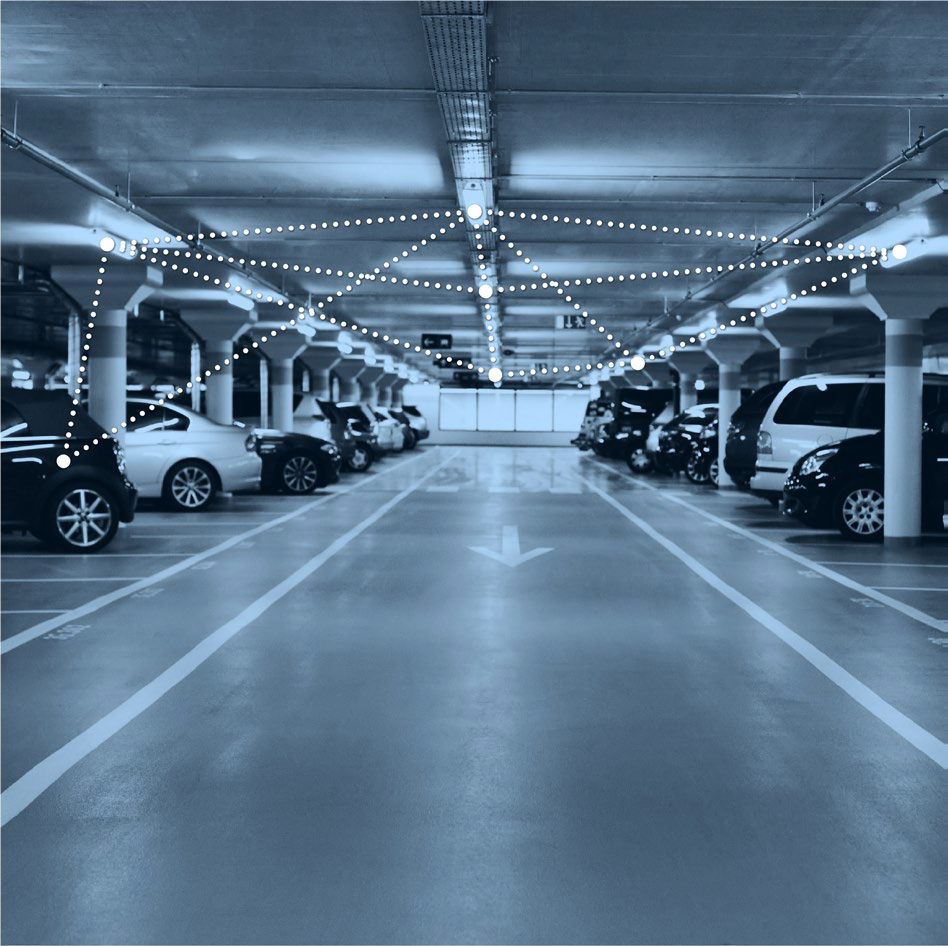
\includegraphics[width=\textwidth]{Bluetooth_Mesh_CarPark_Example.png}
		\caption[Parkhaus mit Bluetooth-Mesh]{Parkhaus mit Bluetooth-Mesh \cite{bluetooth_sig_mesh-technology-overviewpdf_2020}}
		\label{fig:BluetoothMeshParkingExample}
	\end{minipage}
	\begin{minipage}{0.49\textwidth}
		\centering
		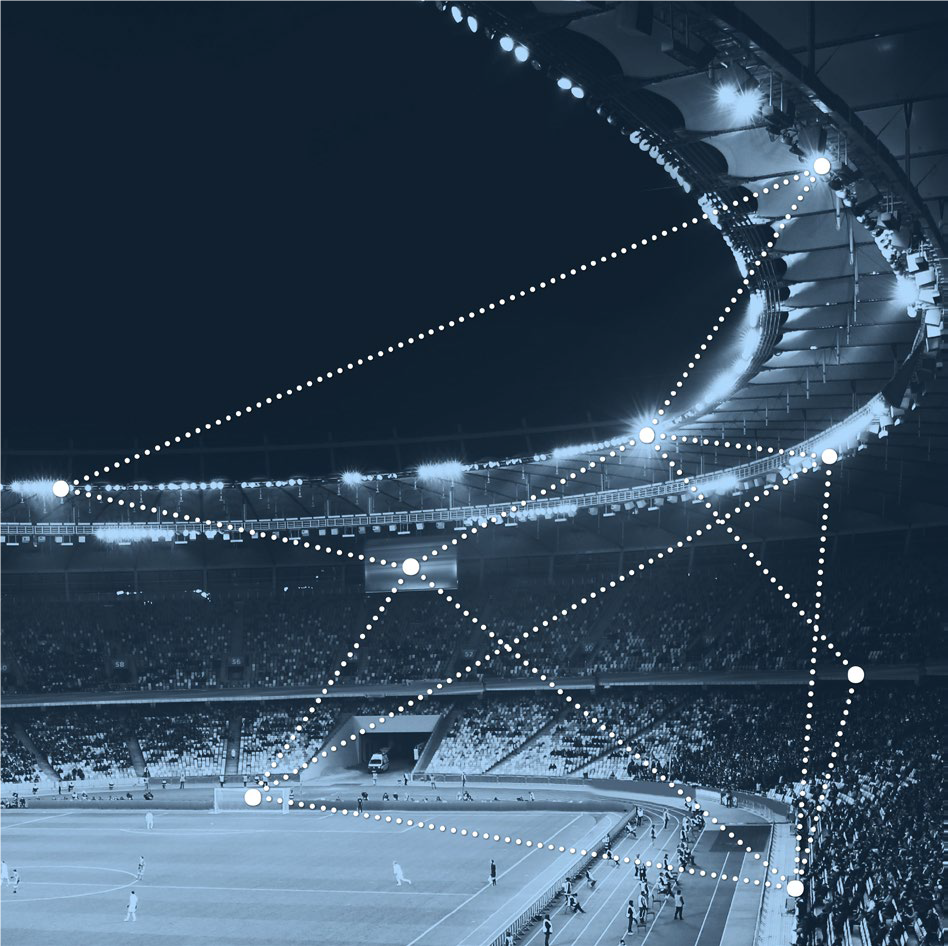
\includegraphics[width=\textwidth]{Bluetooth_Mesh_Stadium_Example.png}
		\caption[Stadion mit Bluetooth-Mesh]{Stadion mit Bluetooth-Mesh \cite{bluetooth_sig_mesh-technology-overviewpdf_2020}}
		\label{fig:BluetoothMeshStadiumExample}
	\end{minipage}
\end{figure}


Die Technologie baut auf den weit verbreitetem BLE-Standard auf, welcher in einer viel zahl von Endgeräten verbaut ist. Ab BLE-Version 4.0 könnten sich die Geräte zu einem Mesh-Netzwerk verbinden. Im Anschluss wird der Netzaufbau kurz erklärt und der Leser mit dem Funktionsprinzip des Mesh-Stacks vertraut gemacht.

Das Einbinden neuer Teilnehmer findet über den Provisioning-Prozess statt. Die Rolle des Provisioners kann ein Smartphone, Laptop oder ein berechtigter Mesh-Teilnehmer übernehmen. Ähnlich wie beim anmelden bei einem WLAN-Netzwerk teilt der Provisioner dem neuen Teilnehmer die Zugangsdaten (Netzwerkschlüssel, etc.) mit. Abschliessend beginnt das neue Gerät im Netzwerk als Node zu operieren. \\  


Bluetooth-Mesh basiert auf dem Managed-Flooding Prinzip. Einfach erklärt wiederholen alle Nodes, abhängig von verschiedenen Bedingungen, jede empfangende Nachricht (Relaying). Somit gelangen die Daten über Zwischenstationen (Hops) zum Ziel. Nachrichten welche nicht für den einzelnen Node relevant sind oder bereits verarbeitet wurden werden verworfen. \\

Um die Funktion von Nodes (Lichtschalter, Lampe, Temperatursensor, etc.) zu unterscheiden, werden sogenannte Models definiert. Jedes Model spezifiziert Zustände (Licht EIN / Licht AUS), welche als States bezeichnet werden. Weiterhin sind Models in drei Kategorien eingeteilt: Server-, Client- und Control-Models. Diese Einteilung schreibt vor ob die Zustände des Nodes zur Veränderung Angeboten werden (Server-Model z.B. Lampe), Zustände verändert werden (Client-Model z.B. Schalter) oder beides möglich ist (Control-Model z.B. Pumpe). Mithilfe dieser Normen lassen sich Geräte von unterschiedlichen Hersteller vereinen, sofern keine Hersteller spezifischen Models verwendet wurden. 

\begin{figure} [H]
	\centering
	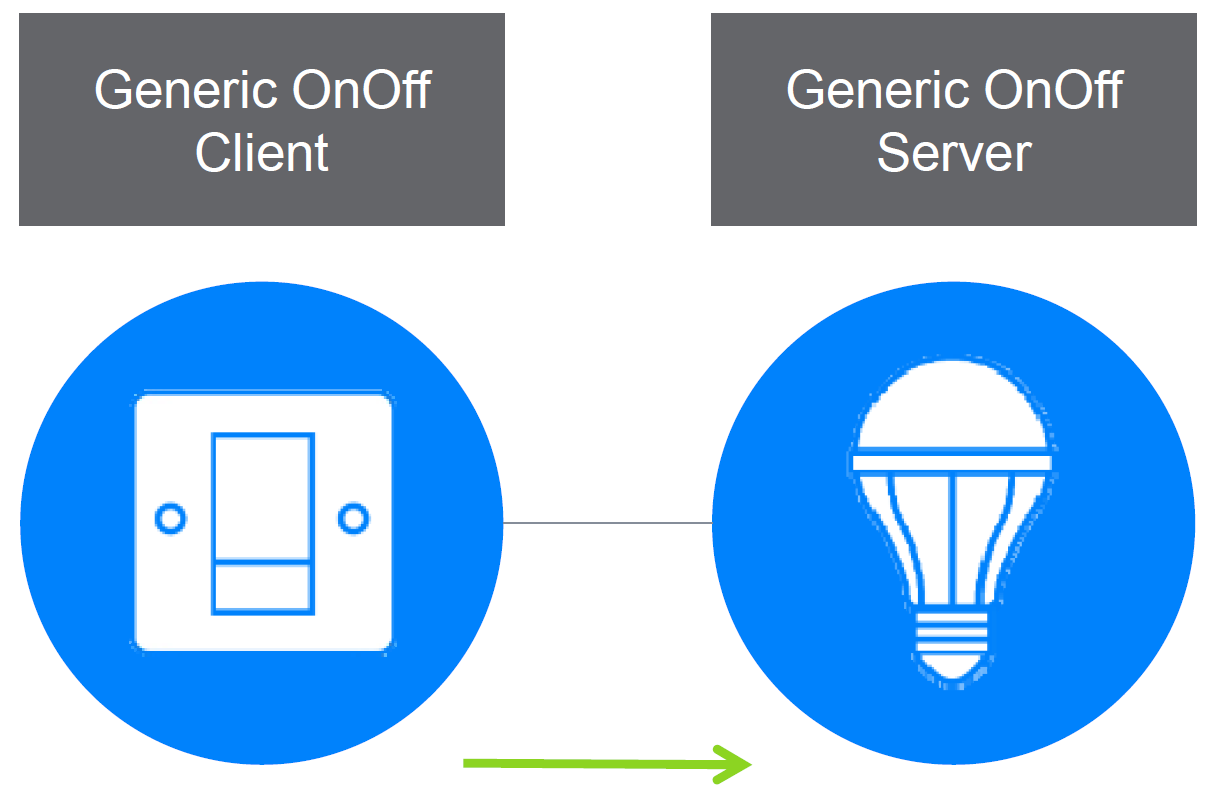
\includegraphics[width=0.6\textwidth]{Bluetooth_Mesh_Client_Server_Prinzip.PNG}
	\caption{Client - Server Prinzip Bluetooth Mesh \cite{bluetooth_sig_mesh-technology-overviewpdf_2020}} 
	\label{fig:BTMeshClientServerPrinzip}
\end{figure}


Zur Identifizierung im Netzwerk besitzt jeder Node eine Unicast-Address (einzigartige Adresse). Um mehrere Nodes zu einer Gruppe zusammenzufassen, werden Group-Addresses vergeben. Die Beziehungen zwischen Nodes werden durch Publishen (Veröffentlichen) oder Subscriben (Abonnieren) auf Adressen geregelt. Im Anwendungsfall Publisht der Client (Schalter) an die Adresse auf welche einer oder mehrere Server (Lampe/Lampen) Subscriben. Wie in Abbildung \ref{fig:BTMeshPublishSubscribePrinzip} ist das Unterscheiden von Bereichen mittels Gruppen möglich. Ein Node kann gleichzeitig an mehrere Adressen Publishen und Subscriben, was zu beliebig komplexen Aufbauten führt. 


\begin{figure} [H]
	\centering
	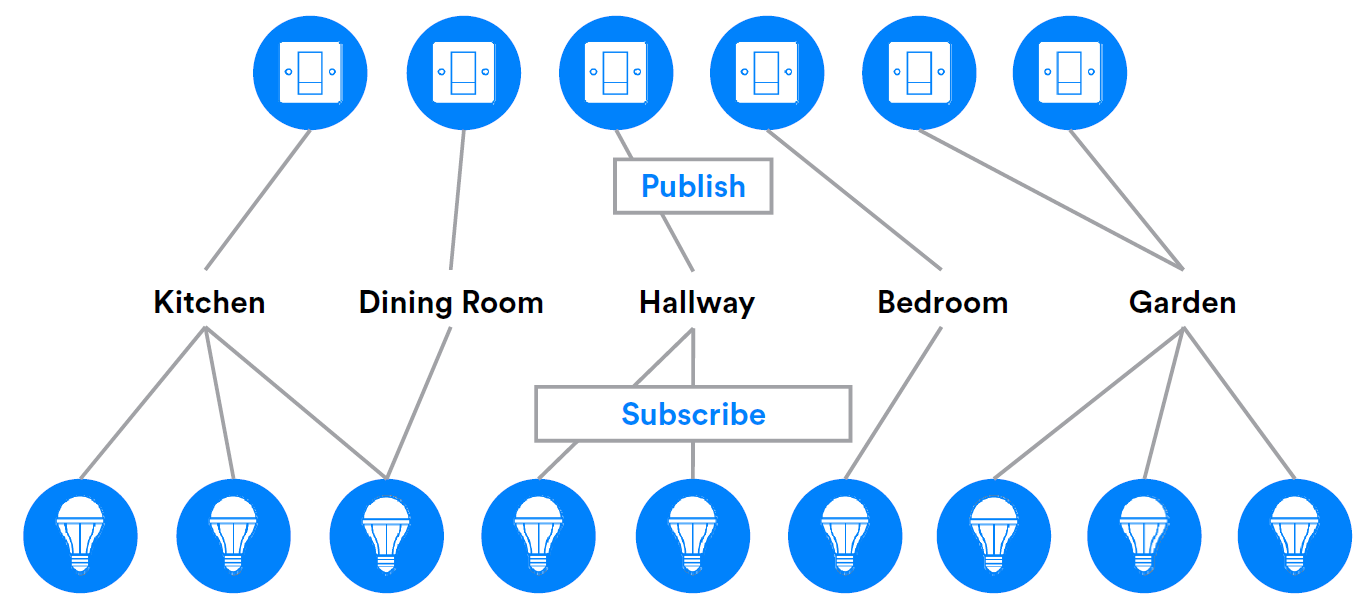
\includegraphics[width=1.0\textwidth]{Bluetooth_Mesh_Publish_Subscribe_Prinzip.PNG}
	\caption{Publish - Subscribe Prinzip Bluetooth Mesh \cite{bluetooth_sig_mesh-technology-overviewpdf_2020}} 
	\label{fig:BTMeshPublishSubscribePrinzip}
\end{figure}









\pagebreak

\clearpage
\section{Lösungskonzept}\label{sec:Loesungskonzept}
Zur Messung und Auswertung der Mesh-Netzwerke dient ein Testframework wie es in Abbildung \ref{fig:KonzeptschemaTestframework} schematisch dargestellt ist.

\begin{figure}[H]
	\centering
	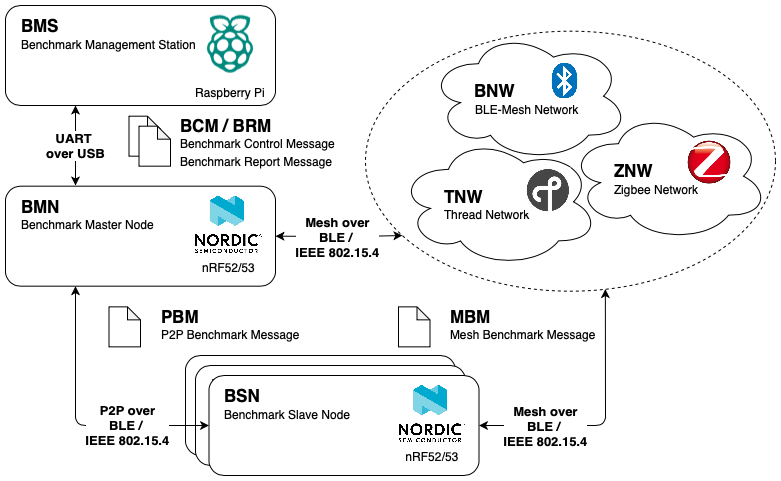
\includegraphics[width=1.0\textwidth]{Konzept_Testframework.jpg}
	\caption{Konzeptschema Testframework}\label{fig:KonzeptschemaTestframework}
\end{figure}


Das Testframework besteht aus folgenden physikalisch getrennten Teilsystemen:

\begin{itemize}
	\item \textbf{BMS} Benchmark Management Station \\ 
	Dient zur Verwaltung und Konfiguration des Testframeworks. Beinhaltet einen Webserver um dem Endanwender die Bedienung zu ermöglichen. Realisiert wird die BMS durch einen \textit{Raspberry Pi 4 Model B}. Als Webserver wird das Python-Framework \textit{Django} eingesetzt. 
	\item \textbf{BMN} Benchmark Master Node \\ 
	Dient als Zugangspunkt der BMS für die im Testframework gefahrenen Tests und lässt sich über eine Serielle Schnittstelle ansprechen. In der Aufgabenstellung \ref{app:Aufgabenstellung} wird der BMN als Master bezeichnet. Realisiert wird der BMN über einen nRF52840 von \textit{Nordic}. 
	\item \textbf{BSN} Benchmark Slave Node \\ 
	Dient als Zugriffspunkt der im Testframework gefahrenen Tests und kann frei in der Testumgebung platziert werden, daher muss die Energieversorgung über einen Akku oder Batterie erfolgen. In der Aufgabenstellung  \ref{app:Aufgabenstellung} wird von einem Slave gesprochen. Realisiert wird der BSN über einen nRF52840 oder nRF5340 von \textit{Nordic}. In einem Test Netzwerk werden unterschiedliche Arten von BSN eingesetzt wie zum Beispiel Mesh Router oder sogenannte End Devices. Letztere werden häufig auch als Low Power Nodes (LPN) bezeichnet.
\end{itemize}

Die logischen Komponenten des Testframeworks lassen sich wie folgt aufteilen:

\begin{itemize}
	\item \textbf{BCM} Benchmark Control Message \\ 
	Beschreibt Nachrichten welche zur Steuerung eines Benchmarks dienen. Dies sind zum Beispiel Konfigurations-, Start- oder Stop-Befehle. Werden von der BMS initiiert und gelangen über eine USB-UART Verbindung zum BMN. 
	\item \textbf{BRM} Benchmark Report Message \\ 
	Beschreibt Nachrichten welche den Status oder die Ergebnisse eines Benchmarks zurückmelden. Werden vom BMN initiiert und gelangen über eine USB-UART Verbindung zur BMS.
	\item \textbf{PBM} P2P Benchmark Message \\ 
	Nachrichten welche während der Durchführung eines Punkt zu Punkt Benchmarks versendet werden. Dies sind zum Beispiel Ping-Anfragen zur Latenzzeitmessung. Sie ermöglichen den Datenaustausch zwischen zwei Teilnehmern auf MAC-Ebene. 
	\item \textbf{MBM} Mesh Benchmark Message \\ 
	Nachrichten welche während der Durchführung eines Mesh Benchmarks versendet werden. Dies sind zum Beispiel Ping-Anfragen zur Latenzzeitmessung. Sie ermöglichen den Datenaustausch über ein Mesh-Netzwerk auf Applikations-Ebene. 
\end{itemize}

\subsection{Punkt zu Punkt Testinfrastruktur}\label{subsec:KonzeptPunktzuPunktTestinfrastruktur}

Die Punkt zu Punkt Testinfrastruktur (P2P) ermöglicht es ein Benchmark auf physikalischer Ebene durchzuführen. Dies soll unabhängig vom Mesh-Protokoll und basierend auf den beiden MAC-Ebenen \textit{BLE} und \textit{IEEE802.15.4} möglich sein. Somit ist ein Vergleich der beiden MAC-Ebenen machbar. Weiter soll diese Infrastruktur einem Endanwender die Möglichkeit bieten die Sende- und Empfangsbedingungen an gegeben Örtlichkeiten auf physikalischer Ebene auszumessen um geeignete Standorte für die Mesh Router zu bestimmen. Die Datenerfassung und grafische Aufbereitung erfolgt dabei auf der BMS. Eine Erfassung der Momentanwerte soll ebenso möglich sein wie die Aufzeichnung der Bedingungen in Form eines Langzeittests über mindestens 24 Stunden.
Schliesslich soll also ein Messinstrument zur Bestimmung der Signalqualitäten im Feld entstehen.
Im Anhang \ref{app:TestKriterienP2P} werden die Testkriterien für die P2P Infrastruktur aufgeführt und beschrieben. Diese Tests werden mit Hilfe bereits bestehenden Beispiel Firmware (Radio-Example) aus der nRF Connect SDK auf dem nRF52840 durchgeführt. Optional wird dies auch noch auf den nRF5340 portiert welcher leistungsfähiger ist.
Weiter soll diese P2P Testinfrastruktur dazu genutzt werden können, gezielte Störungen auf die Test Mesh Netzwerke zu richten die nachfolgend unter \ref{subsec:KonzeptTestMeshNetzwerke} beschrieben werden.


\subsection{Test Mesh Netzwerke}\label{subsec:KonzeptTestMeshNetzwerke}

Der Mesh-Benchmark soll die verschiedenen Mesh-Netzwerke möglichst identisch ausmessen um damit deren Protokoll Stacks untereinander zu vergleichen. Dazu dient bei allen Mesh-Netzwerken die Applikations-Schicht. Ein Mesh Netzwerk wird zwischen dem BMN und den BSN aufgebaut. Dazu werden die einzelnen Nodes über die BMS mit der entsprechenden Firmware geladen und anschliessend im Raum verteilt. Das Laden ist über eine Kabelverbindung (UART) vorgesehen. Allenfalls könnte dies zu einem späteren Zeitpunkt drahtlos mithilfe eines Bootloaders möglich gemacht werden. Dabei handelt es sich jedoch um ein Zusatzziel (siehe \ref{tab:ZusatzzieledesGesamtprojektes}). Die Test Mesh Netzwerke sollen anders als die P2P Testinfrastruktur jedoch nur zu Testzwecken innerhalb dieser Arbeit eingerichtet werden und nicht als Messinstrument für Feldmessungen dienen.
Im Anhang \ref{app:TestKriterienMesh} sind die Testkriterien für den Mesh-Benchmark aufgeführt. Anhand dieser sollen die Messungen durchgeführt und analysiert werden. Zusätzlich sollen die Messungen auch unter verschiedenen Bedingungen durchgeführt werden. Beispielsweise ist zu Erwarten, dass die Messresultate aufgrund von sich verändernder Störbelastung durch andere Geräte in unmittelbarer Nähe unterschiedlich ausfallen, abhängig von Örtlichkeit und Anordnung der Nodes.
Alle drei Mesh Netzwerke verfügen über unterschiedliche Nodetypen mit entsprechend differenzierten Funktionen wie beispielweise Router oder End Devices. Die Mesh Netzwerke sollen möglichst realitätsnahe aufgebaut werden und somit mindestens diese beiden Typen beinhalten. Realitätsnah bedeutet in diesem Kontext dass eine mögliche Anwendung, als Beispiel in der Heimautomation, nachgebaut wird in welcher die Nodetypen und auch die Kommunikationswege klar definiert sind.

\subsubsection{Bluetooth Mesh}\label{subsubsection:Bluetooth Mesh}

Die BLE-Mesh Firmware der Nodes werden aus Beispielen der nRF Connect SDK und Zephyr abgeleitet. Das Mesh-Demo Beispiel erlaubt es die essentiellen Netzwerk Parameter fix vorzugeben. Dadurch müssen die Nodes nicht mehr Provisioniert werden und sind sofort einsatzbereit.


\subsubsection{Thread}\label{subsubsection:Thread} 
Die OpenThread Firmware wird mit Hilfe der API und den Tutorials von der offiziellen OpenThread Webseite erstellt. Die offizielle Seite von Google beschreibt das Netzwerk und alle Informationen die benötigt werden, um eine Firmware zu schreiben.

Die Abbildung \ref{fig:ThreadKonzept} zeigt das Framework des Openthread Netzwerkes auf. Die Kommunikation von der BMS zum BMN findet Seriell mit UART over USB statt. Der Serielle Kanal wird mit Hilfe eines Python-Skripts ausgeführt. 
\begin{figure}[H]
	\centering
	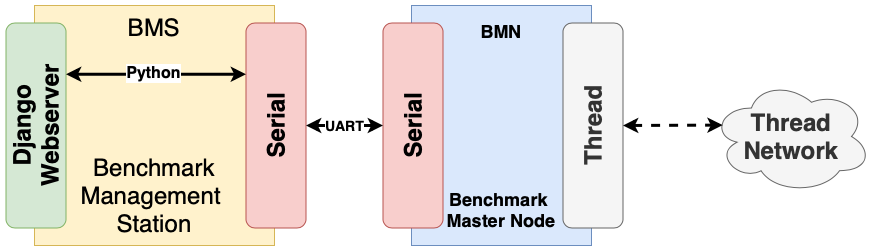
\includegraphics[width=1.0\textwidth]{Thread-Konzept.png}
	\caption{Konzept OpenThread Framework}\label{fig:ThreadKonzept}
\end{figure}


\subsubsection{Zigbee}\label{subsubsection:Zigbee}
Das Zigbee Test Mesh Netzwerk wird mithilfe der \textit{nRF SDK for Thread and Zigbee} eingerichtet und für die Messungen vorbereitet. Der BMN wird dabei als Zigbee Coordinator und gleichzeitig als Zigbee Router eingesetzt. Die BSN können wieder als Router oder aber als Zigbee End Device betrieben werden.

\newpage
\subsection{Steuer und Auswertesoftware}\label{subsec:SteuerundAuswertesoftware}
Die Steuerung des Testframeworks erfolgt über eine Weboberfläche. Diese wird von der BMS mittels WLAN auf den Benutzergeräten zur Anzeige gebracht. Als Webserver dient das Python-Framework \textit{Django}. Zur Steuerung der Benchmarks dienen Schrittketten, welche mit der Firmware auf dem BMN kommunizieren. Als letzter Schritt eines Benchmarks werden die Ergebnisse geloggt, nachbearbeitet und wiederum zur Anzeige gebracht.

Die Abbildung \ref{fig:EntwurfWebserver} stellt ein erstes Konzept dar, wie der Webserver für das P2P Test Framework aussehen kann. Die vom BMN ersichtlichen BSN werden aufgelistet und es können verschiedene  Aktionen durchgeführt werden. Mit Reitern soll auf verschiedene Seiten gewechselt werden auf welchen wiederum Resultate oder Logs der Kommunikation ersichtlich sein sollen.

\begin{figure}[H]
	\centering
	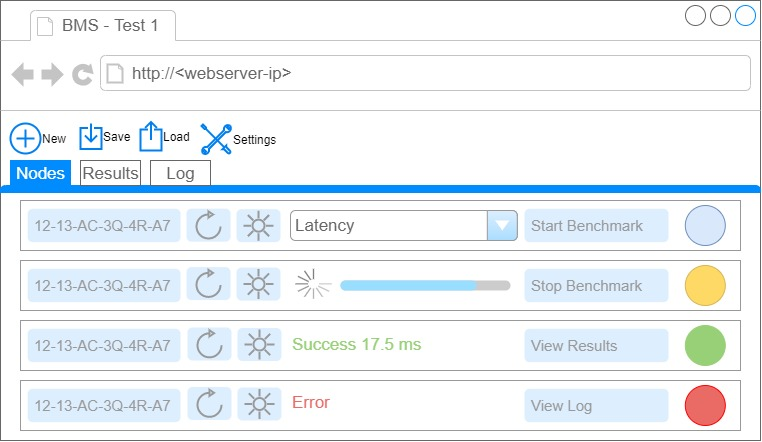
\includegraphics[width=1.0\textwidth]{Web_Mochup_BMS.jpg}
	\caption{Entwurf Webserver}\label{fig:EntwurfWebserver}
\end{figure}


\pagebreak

\clearpage
\section{Projektziele und Lieferobjekte}\label{sec:ProjektzieleundLieferobjekte}

Nachfolgend sind alle Projektziele aufgelistet. Die Ziele wurden in vier Teile unterteilt. Die ersten drei Teile entsprechen den Hauptzielen die in Kapitel \ref{subsec:ZielderArbeit} bereits erwähnt wurden. Die Tabelle \ref{tab:ZusatzzieledesGesamtprojektes} zeigt zusätzliche Ziele die als Wunschziele betrachtet werden und somit nicht im Fokus der Arbeit stehen. Wie bereits unter Kapitel \ref{subsec:KonzeptPunktzuPunktTestinfrastruktur} sowie \ref{subsec:KonzeptTestMeshNetzwerke} erwähnt, sind ergänzende Beschreibungen von Testkriterien in den Anhängen \ref{app:TestKriterienP2P} und \ref{app:TestKriterienMesh} zu finden.

\subsection{Punkt zu Punkt Testinfrastruktur}\label{subsec:PunktzuPunktTestinfrastruktur}

\begin{table}[H]
    \centering
	\begin{tabular}{ | C{0.7cm} | p{3.7cm} | p{10.2cm} |}
		\hline
		\multicolumn{3}{|l|}{\textbf{Projektziele}}\\ \hline
		\textbf{Nr.}& \textbf{Ziel}& \textbf{Beschrieb}\\ \hline
		
		P1 & Kommunikation mit BMS & Der BMN kommuniziert via USB oder UART mit dem BMS.\\ \hline
		
		P2 & Senden von MAC-Frames & Das BMN sendet gemäss den Vorgaben der Testkriterien und gesteuert durch das BMS MAC-Frames an einen oder mehrere BSN.\\ \hline
		
		P3 & Rückbestätigung der MAC-Frames & Der oder die batteriebetriebenen BSN, bestätigen die MAC-Frames mit entsprechender Payload zurück.\\ \hline
		
		P4 & Konfiguration der Anzahl BSN & Die Anzahl der BSN ist über eine Steuer- und Auswertesoftware konfigurierbar.\\ \hline
		
		P5 & Adressierung der BSN & Die Adressierung der BSN ist über eine Steuer- und Auswertesoftware konfigurierbar.\\ \hline
		
		P6 & Konfiguration der Kanäle & Die BLE resp. 802.15.4 Kanäle können über eine Steuer- und Auswertesoftware ausgewählt werden.\\ \hline
		
		P7 & Einstellbare Framelänge & Die Framelänge der MAC-Frames ist über eine Steuer- und Auswertesoftware konfigurierbar.\\ \hline
		
		P8 & Einstellbare Frame- und Kanalwechselrate & Die Frame- und Kanalwechselrate ist über eine Steuer- und Auswertesoftware konfigurierbar.\\ \hline
		
		P9 & Einstellbare Sendeleistung & Die Sendeleistung der BSN ist über eine Steuer- und Auswertesoftware konfigurierbar.\\ \hline
		
		P10 & Anpassung der Modulationsart& In BLE soll die Modulationsart über eine Steuer- und Auswertesoftware konfigurierbar sein, um die Datenrate von 125kbps auf 2Mbps und die Long Range Funktion einzustellen.\\ \hline
		
		P11 & Ein- und Ausschalten der Collision Avoidance (CSMA/CA)& Beim 802.15.4 Protokoll soll die Collision Avoidance über eine Steuer- und Auswertesoftware ein- und ausgeschaltete werden können.\\ \hline
		
		P12 & Erfassen der Verbindungsqualität & Sowohl master- wie auch slaveseitige Erfassung der Verbindungsqualität (RSSI, Package Loss, Collisions, Noise Level, …). Die BSN senden hierzu die erfassten Werte im Rückantwortframe dem BMN zurück. (Siehe auch Anhang \ref{app:TestKriterienP2P})\\ \hline
				
		P13 & Tool für Feldtests & Es soll ein Tool entstehen, welches dem Anwender die Möglichkeit gibt Messungen durchzuführen und somit sein Mesh Netzwerk zu planen.\\ \hline

		
	\end{tabular}\\
	\caption{Projektziele der Punkt zu Punkt Testinfrastruktur}
	\label{tab:ProjektzielederPunktzuPunktTestinfrastruktur}
\end{table}


\subsection{Test Mesh Netzwerke}\label{subsec:TestMeshNetzwerke}
\begin{table}[H]
\centering
	\begin{tabular}{| C{0.7cm} | p{3.7cm} | p{10.2cm} |}
		\hline
		\multicolumn{3}{|l|}{\textbf{Projektziele}}\\ \hline
		\textbf{Nr.}& \textbf{Ziel}& \textbf{Beschrieb}\\ \hline
		
		P1 & Kommunikation mit BMS & Das BMN kommuniziert via USB oder UART mit dem BMS.\\ \hline
		
		P2 &Konfiguration BSN &Die BSN lassen sich frei zu einem Routing-Knoten, End-Knoten oder einem Low-Power Knoten konfigurieren.\\ \hline
		
		P3 & Mesh-Netzwerk & Alle drei Technologien Bluetooth, Thread und Zigbee müssen als Mesh-Netzwerk mit mindestens 10 BSN aufgebaut werden.\\ \hline
		
		P4 & Simulation Sensorwerte & Die BSN sollen in einem vom BMS vorgegebenen parametrisierbaren Intervall Sensorwerte simulieren\\ \hline
		
		P5 & Sensordaten & Als Sensordaten sollen die Netzzustandsdaten übermittelt werden: Paketnummer, Anzahl Retries, Paketverluste, RSSI, Strombedarf und aktive CPU- und Radio-Zeiten.\\ \hline
		
		P6 & Datenauswertung & Die Auswertung der gemessenen Daten soll entweder direkt auf dem BMS oder alternativ auf einem Client Rechner erfolgen. Eine Gegenüberstellung der Daten der drei Mesh Protokolle ist dabei ebenfalls gewünscht.\\ \hline
				
		P7 & Störimmunität & Um die Störimmunität der Netzwerke zu ermitteln sollen gezielt Fremdstörungen  mit definierbarer Tastung und Störframelänge eingebracht werden. Hierfür soll die Punkt zu Punkt Testinfrastruktur auf MAC-Ebene eingesetzt werden.\\ \hline
		
		P8 & Unterschiedliche Test Bedingungen & Die Messungen und Tests an den Mesh Netzwerken sollen unter unterschiedlichen Bedingungen bezüglich Testumgebung durchgeführt werden. Einerseits soll dies in einem Gebäude der FHNW sein und andererseits in einer Umgebung im Heimbereich. \\ \hline
				
		P9 & Test und Validierung & Umfassende Gegenüberstellung und Validierung der Messresultate aller drei Netzwerke. Insbesondere Durchsatz, Antwortzeit, Zuverlässigkeit, Einfachheit der Konfiguration (inkl. Routing), Einfachheit der Ermittlung geeigneter Router-Standorte, Sicherheit und Energieverbrauch.\\ \hline
		
	\end{tabular}\\
	\caption{Projektziele der Test Mesh Netzwerke}
	\label{tab:ProjektzielederTestMeshNetzwerke}
\end{table}


\subsection{Steuer- und Auswertesoftware}\label{subsec:SteuerundAuswertesoftware}
\begin{table}[H]
\centering
	\begin{tabular}{| C{0.7cm} | p{3.7cm} | p{10.2cm} |}
		\hline
		\multicolumn{3}{|l|}{\textbf{Projektziele}}\\ \hline
		\textbf{Nr.}& \textbf{Ziel}& \textbf{Beschrieb}\\ \hline
		
		P1 & Ansteuerung Funkmodul & Das BMS steuert via USB oder UART ein BMN an.\\ \hline
		
		P2 & Visualisierung Parameter& Die Parameter der Ziele von Kapitel \ref{subsec:TestMeshNetzwerke} und \ref{subsec:PunktzuPunktTestinfrastruktur} sollen vom BMS visualisiert und eingestellt werden können.\\ \hline
		
		P3 & User Interface (UI) & Die Testinfrastruktur beinhaltet ein benutzerfreundliches UI.\\ \hline

		
		P4 & Konfiguration Mesh-Netzwerk& Das BMS verwaltet und konfiguriert über einen BMN das Mesh-Netzwerk.\\ \hline
		
		P5 & Einheitliche Kommunikation von BMS & Das Protokoll und Interface zum BMS soll für alle drei Mesh-Netzwerke einheitlich sein.\\ \hline
		
	\end{tabular}\\
	\caption{Projektziele der Steuer- und Auswertesoftware}
	\label{tab:ProjektzielederSteuerundAuswertesoftware}
\end{table}

\subsection{Zusatzziele}\label{subsec:Zusatzziele}
\begin{table}[H]
\centering
	\begin{tabular}{| C{0.7cm} | p{3.7cm} | p{10.2cm} |}
		\hline
		\multicolumn{3}{|l|}{\textbf{Projektziele}}\\ \hline
		\textbf{Nr.}& \textbf{Ziel}& \textbf{Beschrieb}\\ \hline
		
		
		W1 & Hardware Testmodul BMN/BSN & Entwickelung einer eigenen Hardware für das Testmodul mit unabhängiger Stromversorgung und dezidierter Strommessung um den Stromverbrauch aufzuzeichnen.\\ \hline
		
		W2 & Vergleich SOC & Vergleichen zwischen nRF52840, nRF5340 und weiterer kompatibler SOCs.\\ \hline
		
		W3 & Drahtlos Konfiguration & Drahtlose Konfiguration der BSN / BMN Firmware. Somit könnte ein Wechsel zwischen BLE Mesh, Thread und Zigbee während der Runtime möglich werden.\\ \hline
		W4 & UI für Mesh Test & Für die Mesh Tests soll analog zu den P2P Tests ein User Interface implementiert werden.\\ \hline
	
		
	\end{tabular}\\
	\caption{Zusatzziele des Gesamtprojektes}
	\label{tab:ZusatzzieledesGesamtprojektes}
\end{table}



\subsection{Lieferobjekte}\label{subsec:Lieferobjekte}
Zusätzlich zu den Projektzielen, folgen in diesem Kapitel die Lieferobjekte  mit dem jeweiligen Fälligkeitsdatum. In der Tabelle \ref{tbl:Lieferobjekte} sind diese  aufgelistet.  


\begin{table}[H]
     \centering
\begin{tabular}{|c|c|l|}\hline
   \textbf{Nr.} & \textbf{Datum} & \textbf{Lieferobjekt} \\ \hline
   
   1 & 02.03.2020 & Abgabe Pflichtenheft, 1. Version\\ \hline
   2 & 08.03.2020 & Abgabe Pflichtenheft, definitive Version\\ \hline
   3 & 14.08.2020 & Abgabe Fachbericht \\ \hline
   4 & 14.08.2020 & Abgabe Paper \\ \hline
   5 & 14.08.2020 & Abgabe Testaufbau \\ \hline
   6 & 14.08.2020 & Abgabe Factsheet \\ \hline
   7 & 14.08.2020 & Abgabe Poster \\ \hline
   8 & 01.09.2020 & Projektpräsentation \\ \hline
   
 \end{tabular}
     \caption{Lieferobjekte}
     \label{tbl:Lieferobjekte}
\end{table}
\pagebreak

\clearpage
\section{Projektmanagement}\label{sec:Projektmanagement}

Nachfolgend werden die wichtigsten Punkte bezüglich Projektmanagement behandelt. Im Zentrum stehen dabei vor allem die Aufteilung der Zuständigkeiten \ref{subsec:Projektaufteilung} sowie die Projektplanung \ref{subsec:Projektplan}.

Um den Projektfortschritt zu überwachen und allfällige Probleme zu besprechen sind zweiwöchentliche Sitzungen mit den Fachcoaches vorgesehen. Ausserordentliche Termine für Besprechungen werden bei Bedarf zusätzlich definiert.


\subsection{Projektaufteilung}\label{subsec:Projektaufteilung}

Wie bereits im Kapitel \ref{sec:Uebersicht} erwähnt, stellt die vorliegende Projektarbeit die Bachelorthesen von Raffael Anklin, Robin Bobst und Cyrill Horath dar. Die einzelnen Thesen werden grundsätzlich als separate Projekte umgesetzt welche jedoch einen gemeinsamen Teil beinhalten. Innerhalb dieses gemeinsamen Teils welcher als Framework bezeichnet wird, werden die Arbeitspakete dynamisch an die 3 Mitarbeiter verteilt. In der Tabelle \ref{tab:ZuweisungderZustaendigkeiten} ist die genaue Zuweisung der Zuständigkeiten ersichtlich.

\begin{table}[H]
     \centering
     	\begin{tabular}{ | p{2.5cm} | p{6cm} | p{2.7cm} | p{2.8cm} |}\hline
  		\textbf{Bezeichnung} & \textbf{Inhalt} & \textbf{Zuständigkeit} & \textbf{Kennung} \\ \hline
   
   Bluetooth Mesh & Aufbau, Messung und Analyse eines Bluetooth Mesh Netzwerks. & Raffael Anklin & EIT-P-20FS-030\\ \hline
   Thread & Aufbau, Messung und Analyse eines Thread Mesh Netzwerks. & Robin Bobst & EIT-P-20FS-031\\ \hline
   Zigbee & Aufbau, Messung und Analyse eines Zigbee Mesh Netzwerks. & Cyrill Horath & EIT-P-20FS-032 \\ \hline
   Framework & Bereitstellung der Test- und Messinfrastruktur. Dazu gehört der Punkt zu Punkt Testaufbau sowie die Steuer- und Auswertesoftware.  & Alle & - \\ \hline
   
 \end{tabular}
     \caption{Zuweisung der Zuständigkeiten}
     \label{tab:ZuweisungderZustaendigkeiten}
\end{table}





\subsection{Projektplan}\label{subsec:Projektplan}
Die Terminpläne zum Projekt \textit{Wireless Controller for Smart Systems} sind im Anhang zu finden. Sie sind in die 4 Teile unterteilt die in der Projektaufteilung \ref{subsec:Projektaufteilung} behandelt wurden. Unter Anhang \ref{app:Gesamt_Terminplanung} ist der Gesamt Terminplan ersichtlich, welcher unter anderem das Framework sowie Projektmanagement Aufgaben beinhaltet. Die Anhänge \ref{app:Bluetooth_Mesh_Terminplanung}, \ref{app:Thread_Terminplanung} und \ref{app:Zigbee_Terminplanung} sind die Terminpläne für die 3 persönlichen Bachelorthesen.


\subsection{Risikoanalyse}\label{subsec:Risikoanalyse}
Für die Projektarbeit wurde ausserdem eine schlanke Risikoanalyse erstellt. Diese ist in Anhang \ref{app:Risikoanalyse} ersichtlich und soll dem Team bei der Beseitigung von Probleme hilfreich sein.

\newpage
\subsection{Projektvereinbarung}\label{subsec:Projektvereinbarung}

	\begin{tabbing}
		\textbf{Projektcoach und Auftraggeber}\\[0.2cm]
		Di Cerbo Manuel\\[0.2cm]
		Ort, Datum: \hspace{5cm}\=Unterschrift:
		\\[0.5cm]----------------------------- \>-----------------------------
		\\[0.2cm]
		Meier Matthias\\[0.2cm]
		Ort, Datum: \hspace{5cm}\=Unterschrift:
		\\[0.5cm]----------------------------- \>-----------------------------
		\\[1cm]
		\textbf{Projekt: EIT-P-20FS-030}\\[0.2cm]
		Anklin Raffael\\[0.2cm]
		Ort, Datum: \>Unterschrift:
		\\[0.5cm]----------------------------- \>-----------------------------
		\\[0.2cm]
		\textbf{Projekt: EIT-P-20FS-031}\\[0.2cm]		
		Bobst Robin\\[0.2cm]
		Ort, Datum: \>Unterschrift:
		\\[0.5cm]----------------------------- \>-----------------------------
		\\[0.2cm]
		\textbf{Projekt: EIT-P-20FS-032}\\[0.2cm]
		Horath Cyrill\\[0.2cm]
		Ort, Datum: \>Unterschrift:
		\\[0.5cm]----------------------------- \>-----------------------------
	\end{tabbing}
	
	\clearpage
\pagebreak

%%Part 2

	\clearpage
\section{Übersicht}\label{sec:Uebersicht}

Das vorliegende Dokument stellt das Pflichtenheft der Bachelorthesen von Raffael Anklin, Robin Bobst und Cyrill Horath an der Fachhochschule Nordwestschweiz Brugg-Windisch im Studiengang Elektro- und Informationstechnik dar. 
Im kommenden ersten Kapitel soll eine Übersicht über die Ausgangslage sowie das Ziel dieser Arbeit gegeben und somit die Rahmenbedingungen abgesteckt werden. Weiter werden die Lösungskonzepte \ref{sec:Loesungskonzept} sowie die Projektziele und Lieferobjekte \ref{sec:ProjektzieleundLieferobjekte} definiert. Abschliessend soll auch noch das Projektmanagement \ref{sec:Projektmanagement} thematisiert werden. 

\subsection{Ausgangslage}\label{subsec:Ausgangslage}

Unter den standardisierten Low Power Mesh Netzwerk Protokollen im
freien GHz ISM-Band konkurrenzieren sich derzeit vorrangig Bluetooth Mesh, Zigbee sowie Thread.
Bezüglich MAC und Physical Layer basieren Zigbee und Thread auf IEEE 802.15.4 wogegen Bluetooth Mesh auf Bluetooth Low Energy (BLE)
basiert.
Jedes dieser Netzwerkprotokolle hat gewisse Vorzüge: Bluetooth Mesh, dass BLE mittlerweile von jedem Smartphone und Notebook unterstützt wird, Thread aufgrund seiner IPv6 Basis und damit einfachem Übergang ins Internet sowie Zigbee aufgrund seiner etablierten Verbreitung im Smart-Lampenbereich durch Philips, IKEA und Osram.
Hauptproblem aller drei Mesh Netzwerkprotokolle ist nebst physikalisch und distanzbedingter Absorption und Reflexion die Störbeeinflussung durch WLAN (WiFi) und andere Netzwerke im GHz Frequenzbereich.

Im Rahmen des P5 mit dem Namen \textit{Bluetooth-Mesh Plattform für IoT Anwendungen}, wurde das Bluetooth-Mesh Protokoll bereits vertieft betrachtet und dessen Vor- und Nachteile aufgezeigt. Basierend auf diesen Erkenntnissen und Erfahrungen und der oben beschriebenen Thematik soll das Bluetooth-Mesh Protokoll mit den Alternativen Thread sowie Zigbee verglichen werden.

\subsection{Ziel der Arbeit}\label{subsec:ZielderArbeit}

In der vorliegenden Arbeit soll zuerst ein praxistaugliches, einheitliches Testframework für alle drei Mesh Netzwerke erstellt werden, wonach die Tauglichkeit aller drei Mesh Netzwerke unter realitätsnahen Bedingungen ermittelt und verglichen werden soll.
Zwecks besserer Vergleichbarkeit sollen alle drei Testnetze das gleiche Radio-Interface als Grundlage verwenden. Aufgrund der guten
Unterstützung aller drei Mesh Protokolle als auch dem im vergangenen P5 gesammelten Wissens, sollen hierfür die nRF52840 SoCs der Firma Nordic eingesetzt werden. Die zu erstellende Testinfrastruktur soll aus den drei folgenden Teilen bestehen:

\begin{itemize}
 	\item Punkt-Punkt Testinfrastrukturen auf MAC-Ebene
 	\item Test Mesh Netzwerke für BT Mesh, Zigbee und Thread
 	\item Steuer- und Auswertesoftware
\end{itemize}

Die genauen Anforderungen an die Testumgebung sind einerseits in der Aufgabenstellung im Anhang \ref{app:Aufgabenstellung} aufgeführt und andererseits werden sie anhand der Projektziele \ref{sec:ProjektzieleundLieferobjekte} definiert.









\pagebreak

\vspace*{4cm}
\part{Thread}\label{part:Thread}
Robin Bobst
\vspace*{\fill}
\clearpage

\section{Einleitung}\label{sec:EinleitungThread}
Thread ist ein auf IPv6 basiertes Netzwerkprotokoll, das speziell für Internet of Things (IoT) Anwendungen entwickelt wurde. Die einzelnen Teilnehmer im Netzwerk verbinden sich zu einem Mesh-Netzwerk. Wie in der Abbildung \ref{fig:ThreadProtokollLayer} ersichtlich verwendet Thread für eine effiziente Kommunikation mit IPv6-Paketen das Kommunikationsprotokoll 6LoWPAN (IPv6 over Low Power Personal Area Network). 6LoWPAN wendet ein Header-Kompressionsverfahren an, welches es ermöglicht die IPv6-Pakete über den Standard IEEE-802.15.4 zu übermitteln. Dank diesem Standard ist es machbar, die mit Thread entwickelten Geräte so energieeffizient zu gestalten, dass ein Batteriebetrieb realisierbar ist. In der Tabelle \ref{table:MerkmaleThread} sind die wichtigsten Merkmale von Thread aufgelistet. Im Juli 2014 wurde die Thread Working Group ins Leben gerufen, bei der folgende Firmen Bestandteil der Gruppe sind: Nest Labs, Samsung, ARRM Holdings, Qualcom, NXP Semiconductors, Silicon Labs, Big Ass Solutions, Somfy, OSRAM Tyco International und Yale. Ab August 2018 Apple trat auch Apple der Arbeitsgruppe bei, um das Prokoll populär zu machen. \cite[Kapitel 1]{thread_group_inc_thread_2017} \\

\begin{figure}[H]
	\centering
	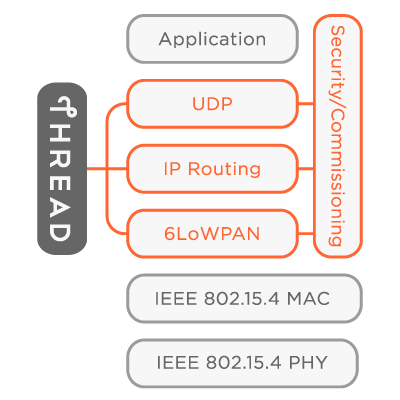
\includegraphics[width=0.5\textwidth]{threadlayerprotocols.png}
	\caption{Thread Protokoll Layer \cite{erickson_picture_2019}}
	\label{fig:ThreadProtokollLayer}
\end{figure}

\begin{table}[H]
	\centering
	\begin{adjustbox}{width=1\textwidth}
	\begin{tabular}{@{}lllll@{}}
		\cmidrule(r){1-2} \cmidrule(l){4-5}
		\multicolumn{2}{|c|}{\textbf{Netzwerk}}                                                              & \multicolumn{1}{l|}{} & \multicolumn{2}{c|}{\textbf{Applikation}}                                                                           \\ \cmidrule(r){1-2} \cmidrule(l){4-5} 
		\multicolumn{1}{|l|}{\textbf{Merkmal}}      & \multicolumn{1}{l|}{\textbf{Beschreibung}}             & \multicolumn{1}{l|}{} & \multicolumn{1}{l|}{\textbf{Merkmal}}                   & \multicolumn{1}{l|}{\textbf{Beschreibung}}                \\ \cmidrule(r){1-2} \cmidrule(l){4-5} 
		\multicolumn{1}{|l|}{IEEE 802.15.4}         & \multicolumn{1}{l|}{Protokoll}                         & \multicolumn{1}{l|}{} & \multicolumn{1}{l|}{IPv6}                               & \multicolumn{1}{l|}{IP-Kommunikation}                     \\ \cmidrule(r){1-2} \cmidrule(l){4-5} 
		\multicolumn{1}{|l|}{MAC Security}          & \multicolumn{1}{l|}{Verschlüsselte Übertragung}        & \multicolumn{1}{l|}{} & \multicolumn{1}{l|}{UDP}                                & \multicolumn{1}{l|}{UDP-Sockets}                          \\ \cmidrule(r){1-2} \cmidrule(l){4-5} 
		\multicolumn{1}{|l|}{6LoWPAN}               & \multicolumn{1}{l|}{Effiziente IPv6 Paket Übertragung} & \multicolumn{1}{l|}{} & \multicolumn{1}{l|}{CoAP}                               & \multicolumn{1}{l|}{Client und Server}                    \\ \cmidrule(r){1-2} \cmidrule(l){4-5} 
		\multicolumn{1}{|l|}{Mesh Routing}          & \multicolumn{1}{l|}{Many-to-many Kommunikation}        & \multicolumn{1}{l|}{} & \multicolumn{1}{l|}{DHCPv6}                             & \multicolumn{1}{l|}{Client und Server}                    \\ \cmidrule(r){1-2} \cmidrule(l){4-5} 
		&                                                        &                       &                                                         &                                                           \\ \cmidrule(r){1-2} \cmidrule(l){4-5} 
		\multicolumn{2}{|c|}{\textbf{Boarder Router}}                                                        & \multicolumn{1}{l|}{} & \multicolumn{2}{c|}{\textbf{Weitere Merkmale}}                                                                      \\ \cmidrule(r){1-2} \cmidrule(l){4-5} 
		\multicolumn{1}{|l|}{Web - UI}              & \multicolumn{1}{l|}{Für Netzwerk Menagement}           & \multicolumn{1}{l|}{} & \multicolumn{1}{l|}{Periodic parent search}             & \multicolumn{1}{l|}{Endgerät wechselt zu besserem Parent} \\ \cmidrule(r){1-2} \cmidrule(l){4-5} 
		\multicolumn{1}{|l|}{Externer Kommissioner} & \multicolumn{1}{l|}{Externes Gerät für Neuaufnahme}    & \multicolumn{1}{l|}{} & \multicolumn{1}{l|}{Jam Detection}                      & \multicolumn{1}{l|}{Signal Stau verhindern}               \\ \cmidrule(r){1-2} \cmidrule(l){4-5} 
		\multicolumn{1}{|l|}{NAT64}                 & \multicolumn{1}{l|}{Kommunikation mit IPv4}            & \multicolumn{1}{l|}{} & \multicolumn{1}{l|}{Child Supervision}                  & \multicolumn{1}{l|}{Endgerät überprüfen}                  \\ \cmidrule(r){1-2} \cmidrule(l){4-5} 
		\multicolumn{1}{|l|}{wpantund}              & \multicolumn{1}{l|}{Interface Treiber}                 & \multicolumn{1}{l|}{} & \multicolumn{1}{l|}{Inform previous parent on reattach} & \multicolumn{1}{l|}{Endgerät Menagement}                  \\ \cmidrule(r){1-2} \cmidrule(l){4-5} 
	\end{tabular}
	\end{adjustbox}
	\caption{Merkmale Thread \cite{thread_group_what_2020}}
	\label{table:MerkmaleThread}
\end{table}


\pagebreak

\clearpage
\section{Lösungskonzept}\label{sec:Loesungskonzept}
Zur Messung und Auswertung der Mesh-Netzwerke dient ein Testframework wie es in Abbildung \ref{fig:KonzeptschemaTestframework} schematisch dargestellt ist.

\begin{figure}[H]
	\centering
	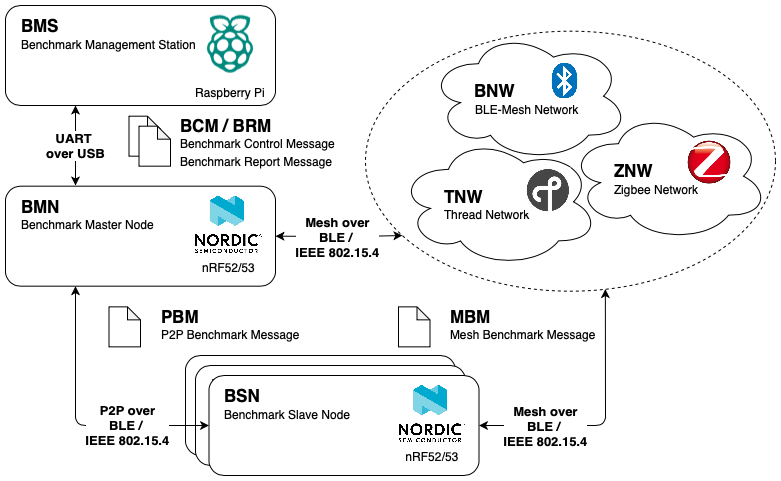
\includegraphics[width=1.0\textwidth]{Konzept_Testframework.jpg}
	\caption{Konzeptschema Testframework}\label{fig:KonzeptschemaTestframework}
\end{figure}


Das Testframework besteht aus folgenden physikalisch getrennten Teilsystemen:

\begin{itemize}
	\item \textbf{BMS} Benchmark Management Station \\ 
	Dient zur Verwaltung und Konfiguration des Testframeworks. Beinhaltet einen Webserver um dem Endanwender die Bedienung zu ermöglichen. Realisiert wird die BMS durch einen \textit{Raspberry Pi 4 Model B}. Als Webserver wird das Python-Framework \textit{Django} eingesetzt. 
	\item \textbf{BMN} Benchmark Master Node \\ 
	Dient als Zugangspunkt der BMS für die im Testframework gefahrenen Tests und lässt sich über eine Serielle Schnittstelle ansprechen. In der Aufgabenstellung \ref{app:Aufgabenstellung} wird der BMN als Master bezeichnet. Realisiert wird der BMN über einen nRF52840 von \textit{Nordic}. 
	\item \textbf{BSN} Benchmark Slave Node \\ 
	Dient als Zugriffspunkt der im Testframework gefahrenen Tests und kann frei in der Testumgebung platziert werden, daher muss die Energieversorgung über einen Akku oder Batterie erfolgen. In der Aufgabenstellung  \ref{app:Aufgabenstellung} wird von einem Slave gesprochen. Realisiert wird der BSN über einen nRF52840 oder nRF5340 von \textit{Nordic}. In einem Test Netzwerk werden unterschiedliche Arten von BSN eingesetzt wie zum Beispiel Mesh Router oder sogenannte End Devices. Letztere werden häufig auch als Low Power Nodes (LPN) bezeichnet.
\end{itemize}

Die logischen Komponenten des Testframeworks lassen sich wie folgt aufteilen:

\begin{itemize}
	\item \textbf{BCM} Benchmark Control Message \\ 
	Beschreibt Nachrichten welche zur Steuerung eines Benchmarks dienen. Dies sind zum Beispiel Konfigurations-, Start- oder Stop-Befehle. Werden von der BMS initiiert und gelangen über eine USB-UART Verbindung zum BMN. 
	\item \textbf{BRM} Benchmark Report Message \\ 
	Beschreibt Nachrichten welche den Status oder die Ergebnisse eines Benchmarks zurückmelden. Werden vom BMN initiiert und gelangen über eine USB-UART Verbindung zur BMS.
	\item \textbf{PBM} P2P Benchmark Message \\ 
	Nachrichten welche während der Durchführung eines Punkt zu Punkt Benchmarks versendet werden. Dies sind zum Beispiel Ping-Anfragen zur Latenzzeitmessung. Sie ermöglichen den Datenaustausch zwischen zwei Teilnehmern auf MAC-Ebene. 
	\item \textbf{MBM} Mesh Benchmark Message \\ 
	Nachrichten welche während der Durchführung eines Mesh Benchmarks versendet werden. Dies sind zum Beispiel Ping-Anfragen zur Latenzzeitmessung. Sie ermöglichen den Datenaustausch über ein Mesh-Netzwerk auf Applikations-Ebene. 
\end{itemize}

\subsection{Punkt zu Punkt Testinfrastruktur}\label{subsec:KonzeptPunktzuPunktTestinfrastruktur}

Die Punkt zu Punkt Testinfrastruktur (P2P) ermöglicht es ein Benchmark auf physikalischer Ebene durchzuführen. Dies soll unabhängig vom Mesh-Protokoll und basierend auf den beiden MAC-Ebenen \textit{BLE} und \textit{IEEE802.15.4} möglich sein. Somit ist ein Vergleich der beiden MAC-Ebenen machbar. Weiter soll diese Infrastruktur einem Endanwender die Möglichkeit bieten die Sende- und Empfangsbedingungen an gegeben Örtlichkeiten auf physikalischer Ebene auszumessen um geeignete Standorte für die Mesh Router zu bestimmen. Die Datenerfassung und grafische Aufbereitung erfolgt dabei auf der BMS. Eine Erfassung der Momentanwerte soll ebenso möglich sein wie die Aufzeichnung der Bedingungen in Form eines Langzeittests über mindestens 24 Stunden.
Schliesslich soll also ein Messinstrument zur Bestimmung der Signalqualitäten im Feld entstehen.
Im Anhang \ref{app:TestKriterienP2P} werden die Testkriterien für die P2P Infrastruktur aufgeführt und beschrieben. Diese Tests werden mit Hilfe bereits bestehenden Beispiel Firmware (Radio-Example) aus der nRF Connect SDK auf dem nRF52840 durchgeführt. Optional wird dies auch noch auf den nRF5340 portiert welcher leistungsfähiger ist.
Weiter soll diese P2P Testinfrastruktur dazu genutzt werden können, gezielte Störungen auf die Test Mesh Netzwerke zu richten die nachfolgend unter \ref{subsec:KonzeptTestMeshNetzwerke} beschrieben werden.


\subsection{Test Mesh Netzwerke}\label{subsec:KonzeptTestMeshNetzwerke}

Der Mesh-Benchmark soll die verschiedenen Mesh-Netzwerke möglichst identisch ausmessen um damit deren Protokoll Stacks untereinander zu vergleichen. Dazu dient bei allen Mesh-Netzwerken die Applikations-Schicht. Ein Mesh Netzwerk wird zwischen dem BMN und den BSN aufgebaut. Dazu werden die einzelnen Nodes über die BMS mit der entsprechenden Firmware geladen und anschliessend im Raum verteilt. Das Laden ist über eine Kabelverbindung (UART) vorgesehen. Allenfalls könnte dies zu einem späteren Zeitpunkt drahtlos mithilfe eines Bootloaders möglich gemacht werden. Dabei handelt es sich jedoch um ein Zusatzziel (siehe \ref{tab:ZusatzzieledesGesamtprojektes}). Die Test Mesh Netzwerke sollen anders als die P2P Testinfrastruktur jedoch nur zu Testzwecken innerhalb dieser Arbeit eingerichtet werden und nicht als Messinstrument für Feldmessungen dienen.
Im Anhang \ref{app:TestKriterienMesh} sind die Testkriterien für den Mesh-Benchmark aufgeführt. Anhand dieser sollen die Messungen durchgeführt und analysiert werden. Zusätzlich sollen die Messungen auch unter verschiedenen Bedingungen durchgeführt werden. Beispielsweise ist zu Erwarten, dass die Messresultate aufgrund von sich verändernder Störbelastung durch andere Geräte in unmittelbarer Nähe unterschiedlich ausfallen, abhängig von Örtlichkeit und Anordnung der Nodes.
Alle drei Mesh Netzwerke verfügen über unterschiedliche Nodetypen mit entsprechend differenzierten Funktionen wie beispielweise Router oder End Devices. Die Mesh Netzwerke sollen möglichst realitätsnahe aufgebaut werden und somit mindestens diese beiden Typen beinhalten. Realitätsnah bedeutet in diesem Kontext dass eine mögliche Anwendung, als Beispiel in der Heimautomation, nachgebaut wird in welcher die Nodetypen und auch die Kommunikationswege klar definiert sind.

\subsubsection{Bluetooth Mesh}\label{subsubsection:Bluetooth Mesh}

Die BLE-Mesh Firmware der Nodes werden aus Beispielen der nRF Connect SDK und Zephyr abgeleitet. Das Mesh-Demo Beispiel erlaubt es die essentiellen Netzwerk Parameter fix vorzugeben. Dadurch müssen die Nodes nicht mehr Provisioniert werden und sind sofort einsatzbereit.


\subsubsection{Thread}\label{subsubsection:Thread} 
Die OpenThread Firmware wird mit Hilfe der API und den Tutorials von der offiziellen OpenThread Webseite erstellt. Die offizielle Seite von Google beschreibt das Netzwerk und alle Informationen die benötigt werden, um eine Firmware zu schreiben.

Die Abbildung \ref{fig:ThreadKonzept} zeigt das Framework des Openthread Netzwerkes auf. Die Kommunikation von der BMS zum BMN findet Seriell mit UART over USB statt. Der Serielle Kanal wird mit Hilfe eines Python-Skripts ausgeführt. 
\begin{figure}[H]
	\centering
	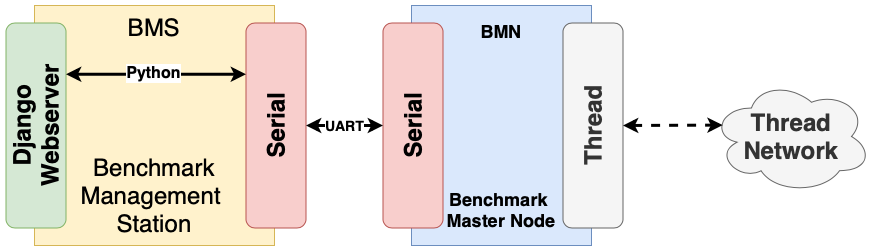
\includegraphics[width=1.0\textwidth]{Thread-Konzept.png}
	\caption{Konzept OpenThread Framework}\label{fig:ThreadKonzept}
\end{figure}


\subsubsection{Zigbee}\label{subsubsection:Zigbee}
Das Zigbee Test Mesh Netzwerk wird mithilfe der \textit{nRF SDK for Thread and Zigbee} eingerichtet und für die Messungen vorbereitet. Der BMN wird dabei als Zigbee Coordinator und gleichzeitig als Zigbee Router eingesetzt. Die BSN können wieder als Router oder aber als Zigbee End Device betrieben werden.

\newpage
\subsection{Steuer und Auswertesoftware}\label{subsec:SteuerundAuswertesoftware}
Die Steuerung des Testframeworks erfolgt über eine Weboberfläche. Diese wird von der BMS mittels WLAN auf den Benutzergeräten zur Anzeige gebracht. Als Webserver dient das Python-Framework \textit{Django}. Zur Steuerung der Benchmarks dienen Schrittketten, welche mit der Firmware auf dem BMN kommunizieren. Als letzter Schritt eines Benchmarks werden die Ergebnisse geloggt, nachbearbeitet und wiederum zur Anzeige gebracht.

Die Abbildung \ref{fig:EntwurfWebserver} stellt ein erstes Konzept dar, wie der Webserver für das P2P Test Framework aussehen kann. Die vom BMN ersichtlichen BSN werden aufgelistet und es können verschiedene  Aktionen durchgeführt werden. Mit Reitern soll auf verschiedene Seiten gewechselt werden auf welchen wiederum Resultate oder Logs der Kommunikation ersichtlich sein sollen.

\begin{figure}[H]
	\centering
	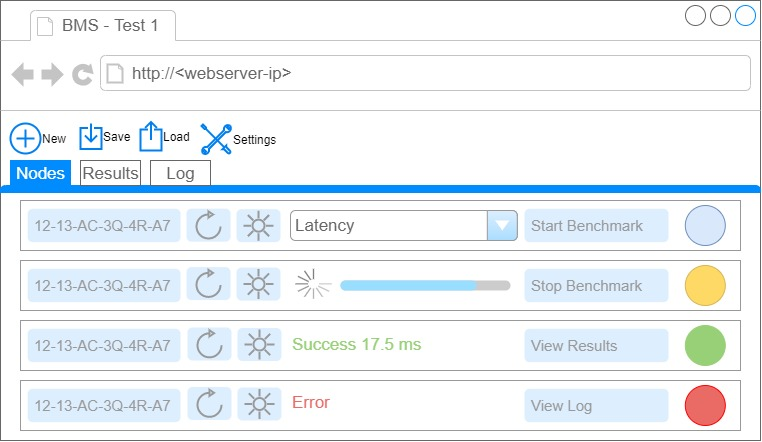
\includegraphics[width=1.0\textwidth]{Web_Mochup_BMS.jpg}
	\caption{Entwurf Webserver}\label{fig:EntwurfWebserver}
\end{figure}


\pagebreak

\clearpage
\section{Projektziele und Lieferobjekte}\label{sec:ProjektzieleundLieferobjekte}

Nachfolgend sind alle Projektziele aufgelistet. Die Ziele wurden in vier Teile unterteilt. Die ersten drei Teile entsprechen den Hauptzielen die in Kapitel \ref{subsec:ZielderArbeit} bereits erwähnt wurden. Die Tabelle \ref{tab:ZusatzzieledesGesamtprojektes} zeigt zusätzliche Ziele die als Wunschziele betrachtet werden und somit nicht im Fokus der Arbeit stehen. Wie bereits unter Kapitel \ref{subsec:KonzeptPunktzuPunktTestinfrastruktur} sowie \ref{subsec:KonzeptTestMeshNetzwerke} erwähnt, sind ergänzende Beschreibungen von Testkriterien in den Anhängen \ref{app:TestKriterienP2P} und \ref{app:TestKriterienMesh} zu finden.

\subsection{Punkt zu Punkt Testinfrastruktur}\label{subsec:PunktzuPunktTestinfrastruktur}

\begin{table}[H]
    \centering
	\begin{tabular}{ | C{0.7cm} | p{3.7cm} | p{10.2cm} |}
		\hline
		\multicolumn{3}{|l|}{\textbf{Projektziele}}\\ \hline
		\textbf{Nr.}& \textbf{Ziel}& \textbf{Beschrieb}\\ \hline
		
		P1 & Kommunikation mit BMS & Der BMN kommuniziert via USB oder UART mit dem BMS.\\ \hline
		
		P2 & Senden von MAC-Frames & Das BMN sendet gemäss den Vorgaben der Testkriterien und gesteuert durch das BMS MAC-Frames an einen oder mehrere BSN.\\ \hline
		
		P3 & Rückbestätigung der MAC-Frames & Der oder die batteriebetriebenen BSN, bestätigen die MAC-Frames mit entsprechender Payload zurück.\\ \hline
		
		P4 & Konfiguration der Anzahl BSN & Die Anzahl der BSN ist über eine Steuer- und Auswertesoftware konfigurierbar.\\ \hline
		
		P5 & Adressierung der BSN & Die Adressierung der BSN ist über eine Steuer- und Auswertesoftware konfigurierbar.\\ \hline
		
		P6 & Konfiguration der Kanäle & Die BLE resp. 802.15.4 Kanäle können über eine Steuer- und Auswertesoftware ausgewählt werden.\\ \hline
		
		P7 & Einstellbare Framelänge & Die Framelänge der MAC-Frames ist über eine Steuer- und Auswertesoftware konfigurierbar.\\ \hline
		
		P8 & Einstellbare Frame- und Kanalwechselrate & Die Frame- und Kanalwechselrate ist über eine Steuer- und Auswertesoftware konfigurierbar.\\ \hline
		
		P9 & Einstellbare Sendeleistung & Die Sendeleistung der BSN ist über eine Steuer- und Auswertesoftware konfigurierbar.\\ \hline
		
		P10 & Anpassung der Modulationsart& In BLE soll die Modulationsart über eine Steuer- und Auswertesoftware konfigurierbar sein, um die Datenrate von 125kbps auf 2Mbps und die Long Range Funktion einzustellen.\\ \hline
		
		P11 & Ein- und Ausschalten der Collision Avoidance (CSMA/CA)& Beim 802.15.4 Protokoll soll die Collision Avoidance über eine Steuer- und Auswertesoftware ein- und ausgeschaltete werden können.\\ \hline
		
		P12 & Erfassen der Verbindungsqualität & Sowohl master- wie auch slaveseitige Erfassung der Verbindungsqualität (RSSI, Package Loss, Collisions, Noise Level, …). Die BSN senden hierzu die erfassten Werte im Rückantwortframe dem BMN zurück. (Siehe auch Anhang \ref{app:TestKriterienP2P})\\ \hline
				
		P13 & Tool für Feldtests & Es soll ein Tool entstehen, welches dem Anwender die Möglichkeit gibt Messungen durchzuführen und somit sein Mesh Netzwerk zu planen.\\ \hline

		
	\end{tabular}\\
	\caption{Projektziele der Punkt zu Punkt Testinfrastruktur}
	\label{tab:ProjektzielederPunktzuPunktTestinfrastruktur}
\end{table}


\subsection{Test Mesh Netzwerke}\label{subsec:TestMeshNetzwerke}
\begin{table}[H]
\centering
	\begin{tabular}{| C{0.7cm} | p{3.7cm} | p{10.2cm} |}
		\hline
		\multicolumn{3}{|l|}{\textbf{Projektziele}}\\ \hline
		\textbf{Nr.}& \textbf{Ziel}& \textbf{Beschrieb}\\ \hline
		
		P1 & Kommunikation mit BMS & Das BMN kommuniziert via USB oder UART mit dem BMS.\\ \hline
		
		P2 &Konfiguration BSN &Die BSN lassen sich frei zu einem Routing-Knoten, End-Knoten oder einem Low-Power Knoten konfigurieren.\\ \hline
		
		P3 & Mesh-Netzwerk & Alle drei Technologien Bluetooth, Thread und Zigbee müssen als Mesh-Netzwerk mit mindestens 10 BSN aufgebaut werden.\\ \hline
		
		P4 & Simulation Sensorwerte & Die BSN sollen in einem vom BMS vorgegebenen parametrisierbaren Intervall Sensorwerte simulieren\\ \hline
		
		P5 & Sensordaten & Als Sensordaten sollen die Netzzustandsdaten übermittelt werden: Paketnummer, Anzahl Retries, Paketverluste, RSSI, Strombedarf und aktive CPU- und Radio-Zeiten.\\ \hline
		
		P6 & Datenauswertung & Die Auswertung der gemessenen Daten soll entweder direkt auf dem BMS oder alternativ auf einem Client Rechner erfolgen. Eine Gegenüberstellung der Daten der drei Mesh Protokolle ist dabei ebenfalls gewünscht.\\ \hline
				
		P7 & Störimmunität & Um die Störimmunität der Netzwerke zu ermitteln sollen gezielt Fremdstörungen  mit definierbarer Tastung und Störframelänge eingebracht werden. Hierfür soll die Punkt zu Punkt Testinfrastruktur auf MAC-Ebene eingesetzt werden.\\ \hline
		
		P8 & Unterschiedliche Test Bedingungen & Die Messungen und Tests an den Mesh Netzwerken sollen unter unterschiedlichen Bedingungen bezüglich Testumgebung durchgeführt werden. Einerseits soll dies in einem Gebäude der FHNW sein und andererseits in einer Umgebung im Heimbereich. \\ \hline
				
		P9 & Test und Validierung & Umfassende Gegenüberstellung und Validierung der Messresultate aller drei Netzwerke. Insbesondere Durchsatz, Antwortzeit, Zuverlässigkeit, Einfachheit der Konfiguration (inkl. Routing), Einfachheit der Ermittlung geeigneter Router-Standorte, Sicherheit und Energieverbrauch.\\ \hline
		
	\end{tabular}\\
	\caption{Projektziele der Test Mesh Netzwerke}
	\label{tab:ProjektzielederTestMeshNetzwerke}
\end{table}


\subsection{Steuer- und Auswertesoftware}\label{subsec:SteuerundAuswertesoftware}
\begin{table}[H]
\centering
	\begin{tabular}{| C{0.7cm} | p{3.7cm} | p{10.2cm} |}
		\hline
		\multicolumn{3}{|l|}{\textbf{Projektziele}}\\ \hline
		\textbf{Nr.}& \textbf{Ziel}& \textbf{Beschrieb}\\ \hline
		
		P1 & Ansteuerung Funkmodul & Das BMS steuert via USB oder UART ein BMN an.\\ \hline
		
		P2 & Visualisierung Parameter& Die Parameter der Ziele von Kapitel \ref{subsec:TestMeshNetzwerke} und \ref{subsec:PunktzuPunktTestinfrastruktur} sollen vom BMS visualisiert und eingestellt werden können.\\ \hline
		
		P3 & User Interface (UI) & Die Testinfrastruktur beinhaltet ein benutzerfreundliches UI.\\ \hline

		
		P4 & Konfiguration Mesh-Netzwerk& Das BMS verwaltet und konfiguriert über einen BMN das Mesh-Netzwerk.\\ \hline
		
		P5 & Einheitliche Kommunikation von BMS & Das Protokoll und Interface zum BMS soll für alle drei Mesh-Netzwerke einheitlich sein.\\ \hline
		
	\end{tabular}\\
	\caption{Projektziele der Steuer- und Auswertesoftware}
	\label{tab:ProjektzielederSteuerundAuswertesoftware}
\end{table}

\subsection{Zusatzziele}\label{subsec:Zusatzziele}
\begin{table}[H]
\centering
	\begin{tabular}{| C{0.7cm} | p{3.7cm} | p{10.2cm} |}
		\hline
		\multicolumn{3}{|l|}{\textbf{Projektziele}}\\ \hline
		\textbf{Nr.}& \textbf{Ziel}& \textbf{Beschrieb}\\ \hline
		
		
		W1 & Hardware Testmodul BMN/BSN & Entwickelung einer eigenen Hardware für das Testmodul mit unabhängiger Stromversorgung und dezidierter Strommessung um den Stromverbrauch aufzuzeichnen.\\ \hline
		
		W2 & Vergleich SOC & Vergleichen zwischen nRF52840, nRF5340 und weiterer kompatibler SOCs.\\ \hline
		
		W3 & Drahtlos Konfiguration & Drahtlose Konfiguration der BSN / BMN Firmware. Somit könnte ein Wechsel zwischen BLE Mesh, Thread und Zigbee während der Runtime möglich werden.\\ \hline
		W4 & UI für Mesh Test & Für die Mesh Tests soll analog zu den P2P Tests ein User Interface implementiert werden.\\ \hline
	
		
	\end{tabular}\\
	\caption{Zusatzziele des Gesamtprojektes}
	\label{tab:ZusatzzieledesGesamtprojektes}
\end{table}



\subsection{Lieferobjekte}\label{subsec:Lieferobjekte}
Zusätzlich zu den Projektzielen, folgen in diesem Kapitel die Lieferobjekte  mit dem jeweiligen Fälligkeitsdatum. In der Tabelle \ref{tbl:Lieferobjekte} sind diese  aufgelistet.  


\begin{table}[H]
     \centering
\begin{tabular}{|c|c|l|}\hline
   \textbf{Nr.} & \textbf{Datum} & \textbf{Lieferobjekt} \\ \hline
   
   1 & 02.03.2020 & Abgabe Pflichtenheft, 1. Version\\ \hline
   2 & 08.03.2020 & Abgabe Pflichtenheft, definitive Version\\ \hline
   3 & 14.08.2020 & Abgabe Fachbericht \\ \hline
   4 & 14.08.2020 & Abgabe Paper \\ \hline
   5 & 14.08.2020 & Abgabe Testaufbau \\ \hline
   6 & 14.08.2020 & Abgabe Factsheet \\ \hline
   7 & 14.08.2020 & Abgabe Poster \\ \hline
   8 & 01.09.2020 & Projektpräsentation \\ \hline
   
 \end{tabular}
     \caption{Lieferobjekte}
     \label{tbl:Lieferobjekte}
\end{table}
\pagebreak

\clearpage
\section{Projektmanagement}\label{sec:Projektmanagement}

Nachfolgend werden die wichtigsten Punkte bezüglich Projektmanagement behandelt. Im Zentrum stehen dabei vor allem die Aufteilung der Zuständigkeiten \ref{subsec:Projektaufteilung} sowie die Projektplanung \ref{subsec:Projektplan}.

Um den Projektfortschritt zu überwachen und allfällige Probleme zu besprechen sind zweiwöchentliche Sitzungen mit den Fachcoaches vorgesehen. Ausserordentliche Termine für Besprechungen werden bei Bedarf zusätzlich definiert.


\subsection{Projektaufteilung}\label{subsec:Projektaufteilung}

Wie bereits im Kapitel \ref{sec:Uebersicht} erwähnt, stellt die vorliegende Projektarbeit die Bachelorthesen von Raffael Anklin, Robin Bobst und Cyrill Horath dar. Die einzelnen Thesen werden grundsätzlich als separate Projekte umgesetzt welche jedoch einen gemeinsamen Teil beinhalten. Innerhalb dieses gemeinsamen Teils welcher als Framework bezeichnet wird, werden die Arbeitspakete dynamisch an die 3 Mitarbeiter verteilt. In der Tabelle \ref{tab:ZuweisungderZustaendigkeiten} ist die genaue Zuweisung der Zuständigkeiten ersichtlich.

\begin{table}[H]
     \centering
     	\begin{tabular}{ | p{2.5cm} | p{6cm} | p{2.7cm} | p{2.8cm} |}\hline
  		\textbf{Bezeichnung} & \textbf{Inhalt} & \textbf{Zuständigkeit} & \textbf{Kennung} \\ \hline
   
   Bluetooth Mesh & Aufbau, Messung und Analyse eines Bluetooth Mesh Netzwerks. & Raffael Anklin & EIT-P-20FS-030\\ \hline
   Thread & Aufbau, Messung und Analyse eines Thread Mesh Netzwerks. & Robin Bobst & EIT-P-20FS-031\\ \hline
   Zigbee & Aufbau, Messung und Analyse eines Zigbee Mesh Netzwerks. & Cyrill Horath & EIT-P-20FS-032 \\ \hline
   Framework & Bereitstellung der Test- und Messinfrastruktur. Dazu gehört der Punkt zu Punkt Testaufbau sowie die Steuer- und Auswertesoftware.  & Alle & - \\ \hline
   
 \end{tabular}
     \caption{Zuweisung der Zuständigkeiten}
     \label{tab:ZuweisungderZustaendigkeiten}
\end{table}





\subsection{Projektplan}\label{subsec:Projektplan}
Die Terminpläne zum Projekt \textit{Wireless Controller for Smart Systems} sind im Anhang zu finden. Sie sind in die 4 Teile unterteilt die in der Projektaufteilung \ref{subsec:Projektaufteilung} behandelt wurden. Unter Anhang \ref{app:Gesamt_Terminplanung} ist der Gesamt Terminplan ersichtlich, welcher unter anderem das Framework sowie Projektmanagement Aufgaben beinhaltet. Die Anhänge \ref{app:Bluetooth_Mesh_Terminplanung}, \ref{app:Thread_Terminplanung} und \ref{app:Zigbee_Terminplanung} sind die Terminpläne für die 3 persönlichen Bachelorthesen.


\subsection{Risikoanalyse}\label{subsec:Risikoanalyse}
Für die Projektarbeit wurde ausserdem eine schlanke Risikoanalyse erstellt. Diese ist in Anhang \ref{app:Risikoanalyse} ersichtlich und soll dem Team bei der Beseitigung von Probleme hilfreich sein.

\newpage
\subsection{Projektvereinbarung}\label{subsec:Projektvereinbarung}

	\begin{tabbing}
		\textbf{Projektcoach und Auftraggeber}\\[0.2cm]
		Di Cerbo Manuel\\[0.2cm]
		Ort, Datum: \hspace{5cm}\=Unterschrift:
		\\[0.5cm]----------------------------- \>-----------------------------
		\\[0.2cm]
		Meier Matthias\\[0.2cm]
		Ort, Datum: \hspace{5cm}\=Unterschrift:
		\\[0.5cm]----------------------------- \>-----------------------------
		\\[1cm]
		\textbf{Projekt: EIT-P-20FS-030}\\[0.2cm]
		Anklin Raffael\\[0.2cm]
		Ort, Datum: \>Unterschrift:
		\\[0.5cm]----------------------------- \>-----------------------------
		\\[0.2cm]
		\textbf{Projekt: EIT-P-20FS-031}\\[0.2cm]		
		Bobst Robin\\[0.2cm]
		Ort, Datum: \>Unterschrift:
		\\[0.5cm]----------------------------- \>-----------------------------
		\\[0.2cm]
		\textbf{Projekt: EIT-P-20FS-032}\\[0.2cm]
		Horath Cyrill\\[0.2cm]
		Ort, Datum: \>Unterschrift:
		\\[0.5cm]----------------------------- \>-----------------------------
	\end{tabbing}
	
	\clearpage
\pagebreak

\clearpage
%%---BIBLIOGRAPHY------------------------------------------------------------------------
{\sloppypar
\printbibliography[heading=bibintoc]
\label{sec:lit}
%\selectlanguage{ngerman}				%ngerman or english
%\printbibliography
}

%%---APPENDIX----------------------------------------------------------------------------
\begin{appendix} 

\addcontentsline{toc}{section}{Anhang}


%**********************Aufgabenstellung***************************
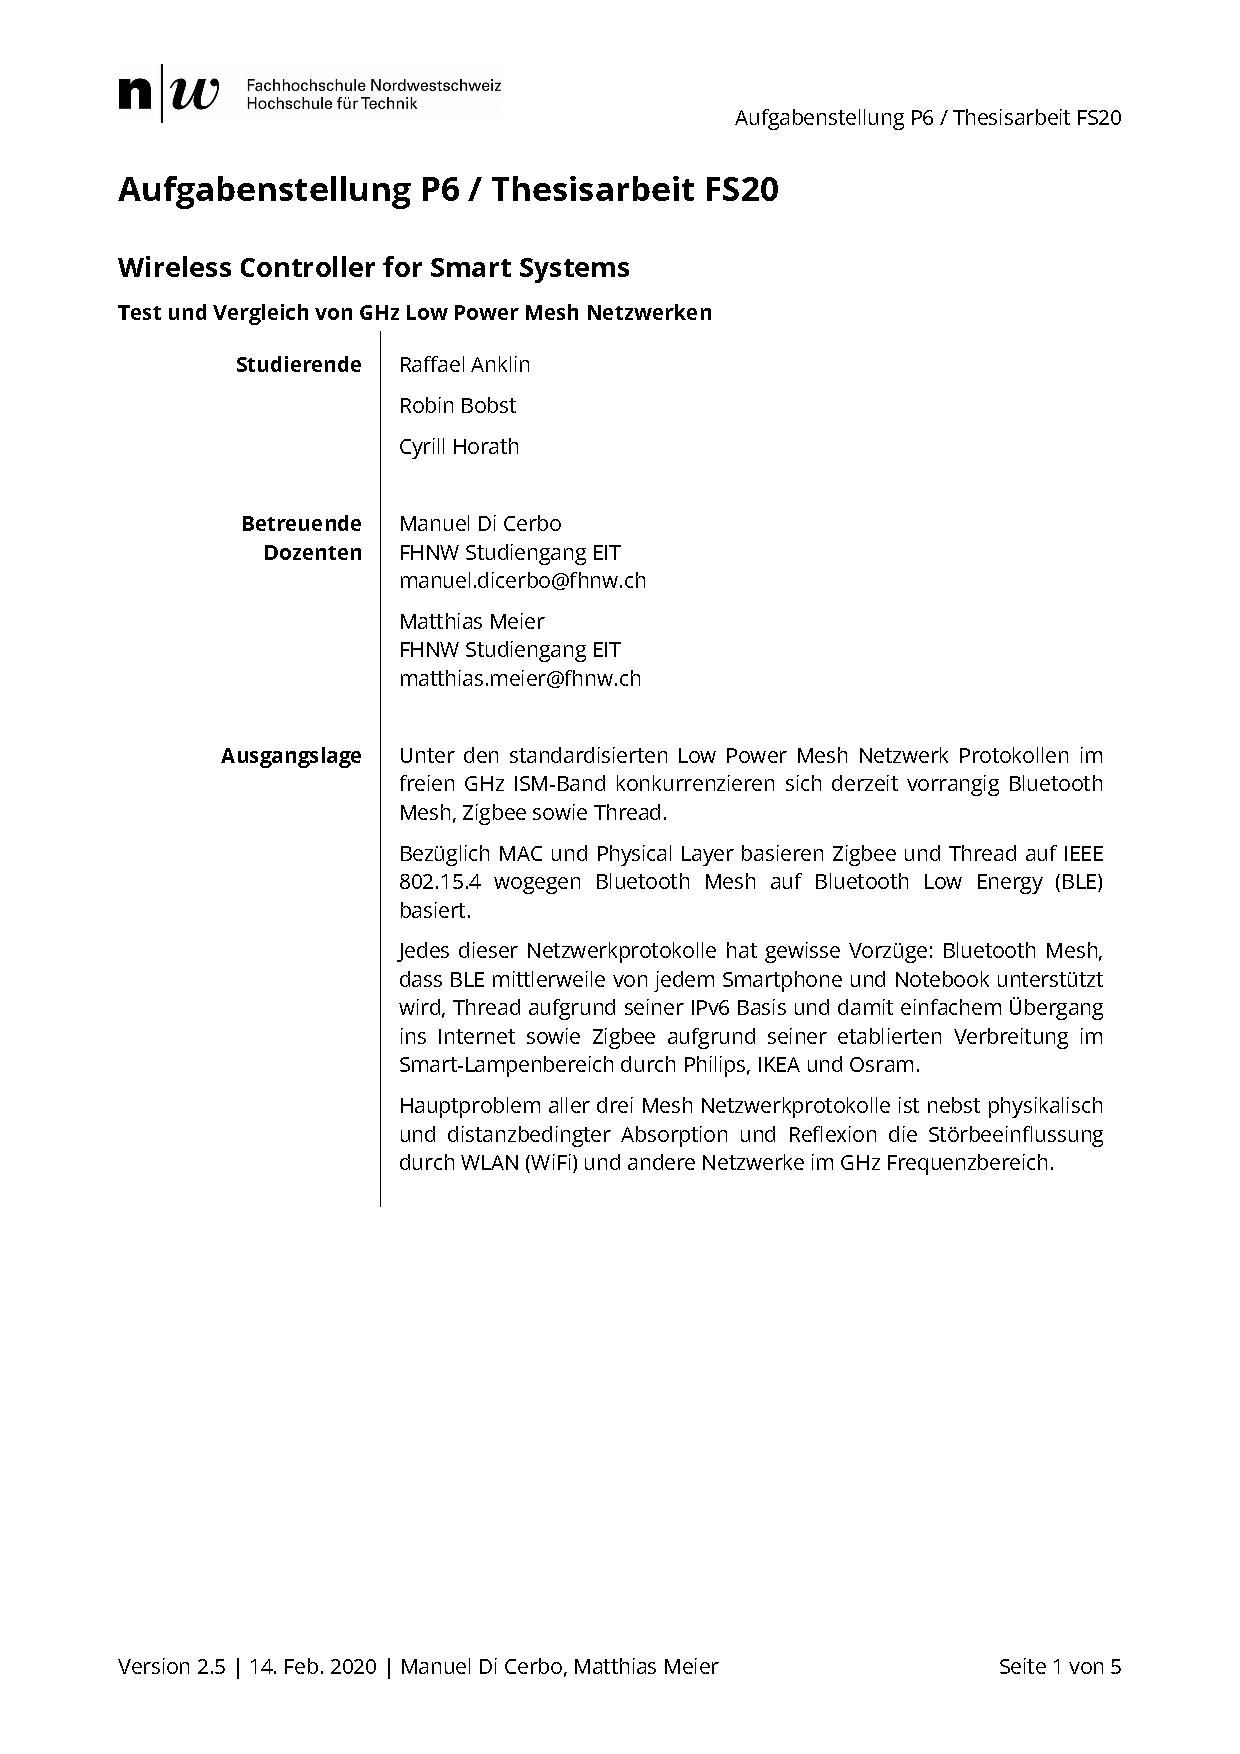
\includepdf[pages={1}, nup=1x1, landscape=false, scale=0.9 ,offset=0 -45, pagecommand={\section{Aufgabenstellung}\label{app:Aufgabenstellung}\thispagestyle{myheadings}}]{appendix/P6_Aufgabenstellung_Wireless_Controller_for_Smart_Systems.pdf}

\includepdf[pages={2-5}, nup=1x1, landscape=false, scale=0.9 ,offset=0 -45, pagecommand={\thispagestyle{myheadings}}]{appendix/P6_Aufgabenstellung_Wireless_Controller_for_Smart_Systems.pdf}


%**********************Pflichtenheft***************************

\includepdf[pages={1}, nup=1x1, landscape=false, scale=0.95 ,offset=0 -45, pagecommand={\section{Pflichtenheft}\label{app:Pflichtenheft}\thispagestyle{myheadings}}]{appendix/P6_Pflichtenheft.pdf}


\includepdf[pages={2-19}, nup=1x1, landscape=false, scale=0.95 ,offset=0 -45, pagecommand={\thispagestyle{myheadings}}]{appendix/P6_Pflichtenheft.pdf}

%***************EMV Bericht Abstrahlung Antennen*********************
\includepdf[pages={1}, nup=1x1, landscape=false, scale=0.95 ,offset=0 -45, pagecommand={\section{Bericht emv Messung Development Kits}\label{app:BerichtemvMessungDevelopmentKits}\thispagestyle{myheadings}}]{appendix/emv_Bericht_FS20.pdf}

\includepdf[pages={2-13}, nup=1x1, landscape=false, scale=0.95 ,offset=0 0, pagecommand={\thispagestyle{myheadings}}]{appendix/emv_Bericht_FS20.pdf}

%***************Messprotokolle Mesh Benchmark*********************
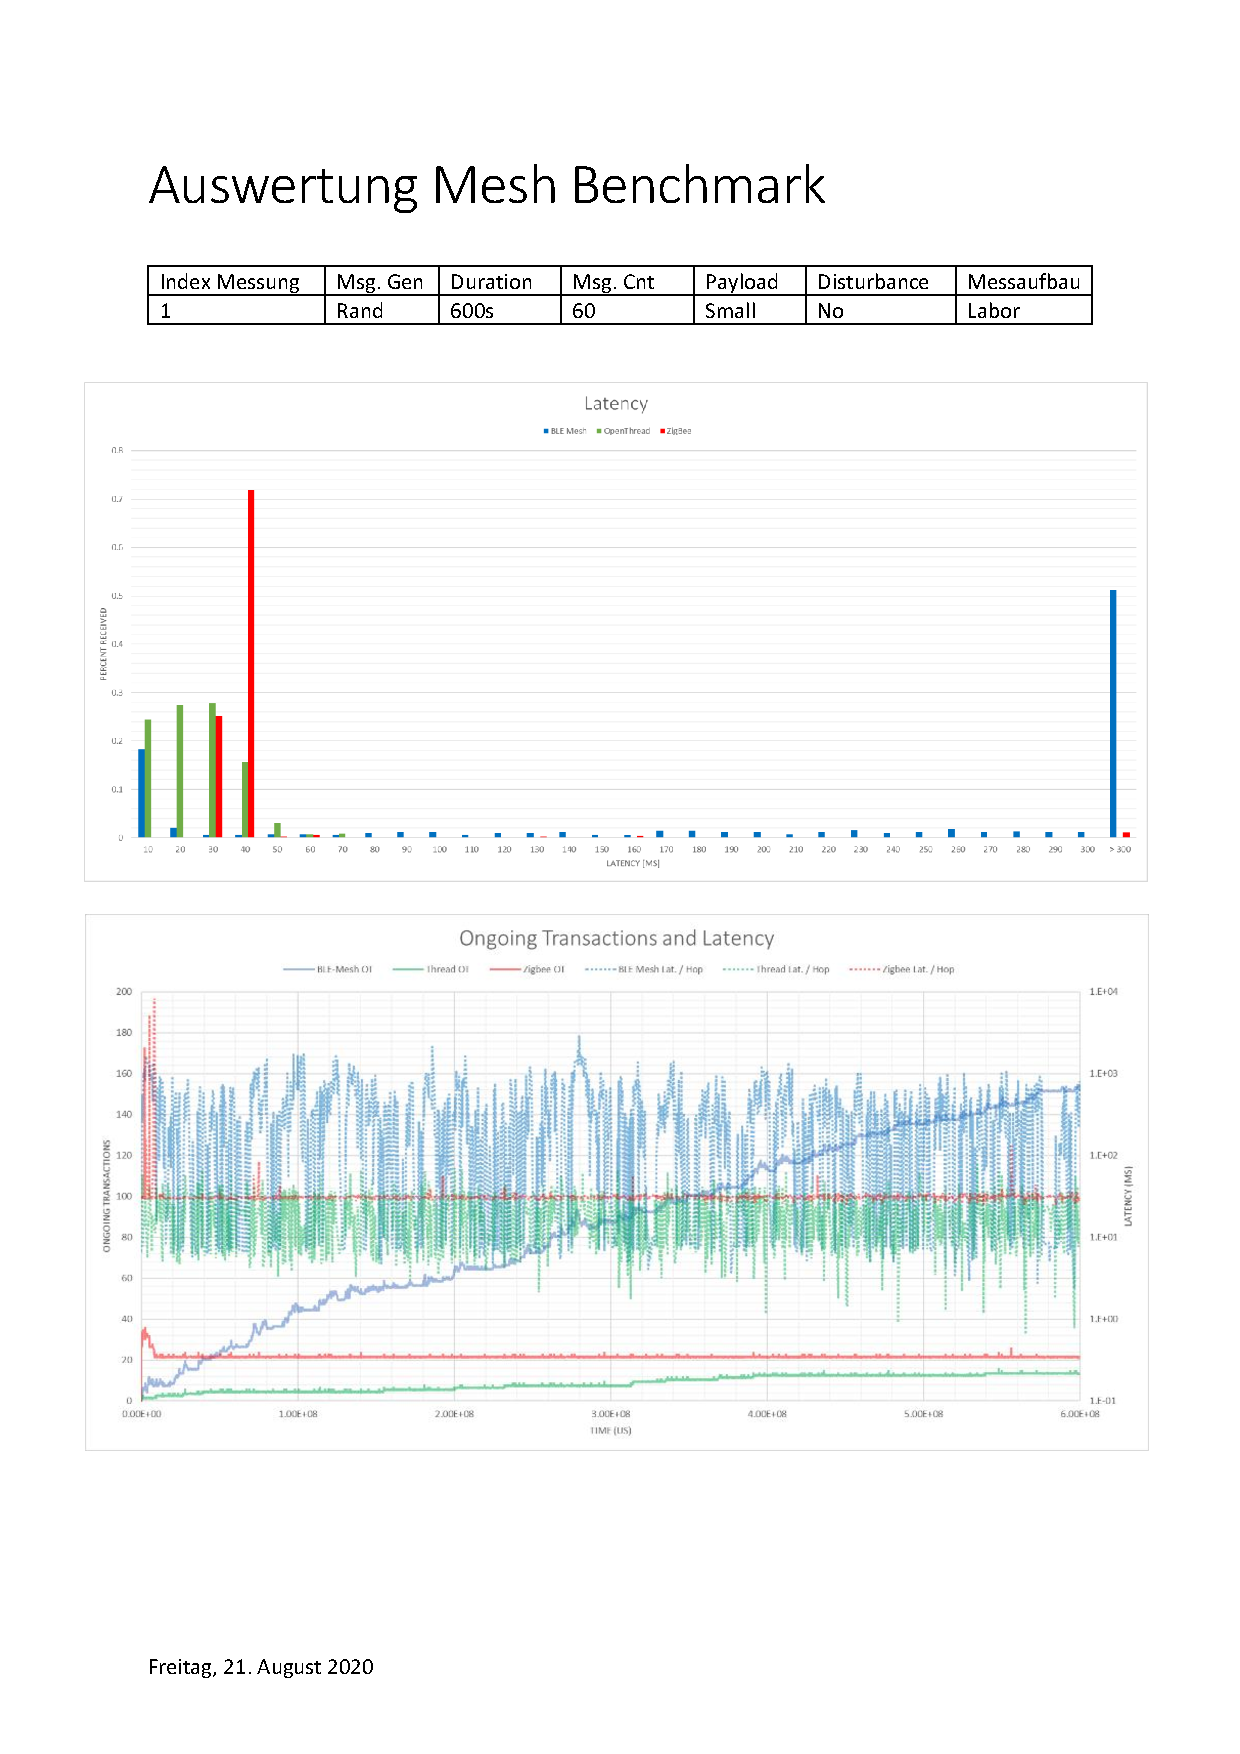
\includepdf[pages={1}, nup=1x1, landscape=false, scale=0.95 ,offset=0 -20, pagecommand={\section{Messprotokolle Mesh Benchmark}\label{app:MessprotokolleMeshBenchmark}\thispagestyle{myheadings}}]{appendix/Messprotokolle_Labor.pdf}

\includepdf[pages={2-14}, nup=1x1, landscape=false, scale=0.95 ,offset=0 0, pagecommand={\thispagestyle{myheadings}}]{appendix/Messprotokolle_Labor.pdf}

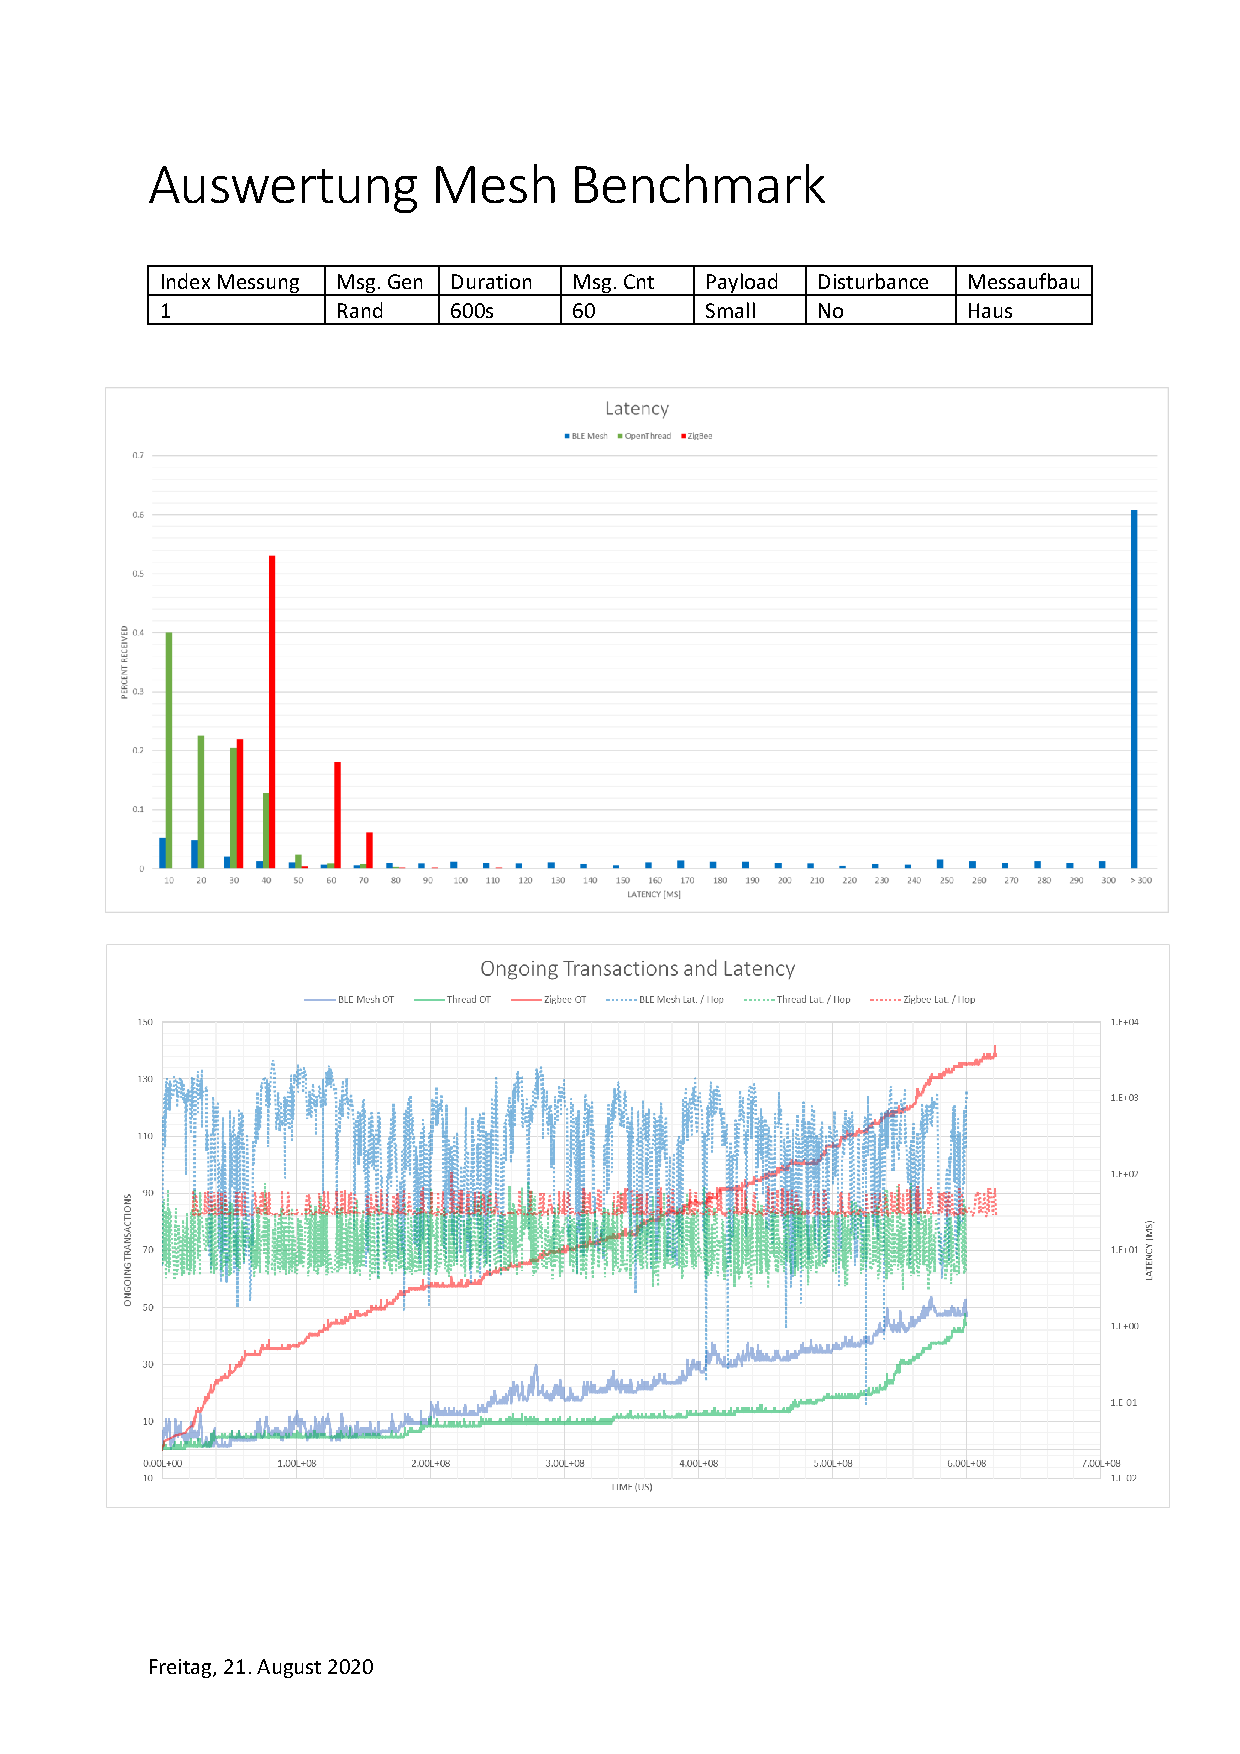
\includepdf[pages={1}, nup=1x1, landscape=false, scale=0.95 ,offset=0 0, pagecommand={\thispagestyle{myheadings}}]{appendix/Messprotokolle_Haus.pdf}

\includepdf[pages={2-8}, nup=1x1, landscape=false, scale=0.95 ,offset=0 0, pagecommand={\thispagestyle{myheadings}}]{appendix/Messprotokolle_Haus.pdf}

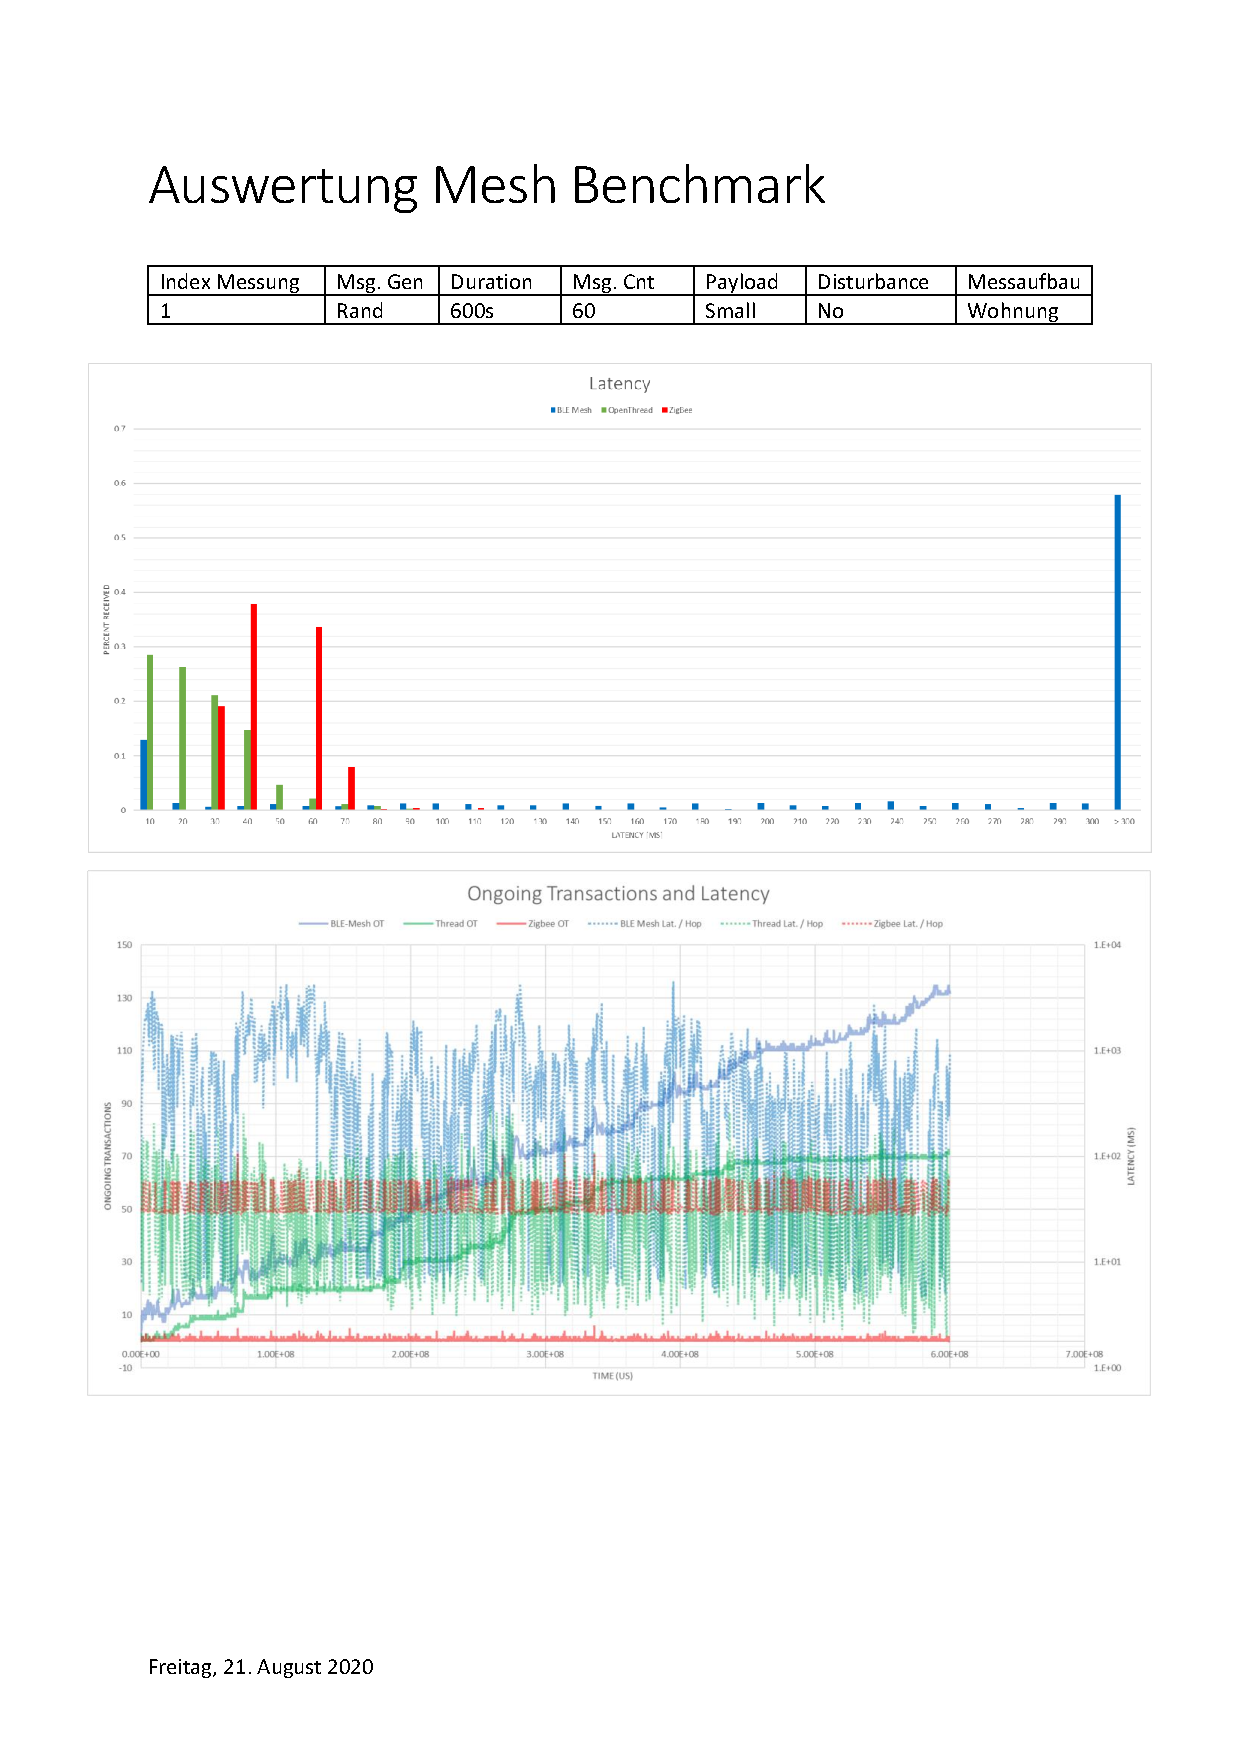
\includepdf[pages={1}, nup=1x1, landscape=false, scale=0.95 ,offset=0 0, pagecommand={\thispagestyle{myheadings}}]{appendix/Messprotokolle_Wohnung.pdf}

\includepdf[pages={2-8}, nup=1x1, landscape=false, scale=0.95 ,offset=0 0, pagecommand={\thispagestyle{myheadings}}]{appendix/Messprotokolle_Wohnung.pdf}

%***************Random Value Generation*********************
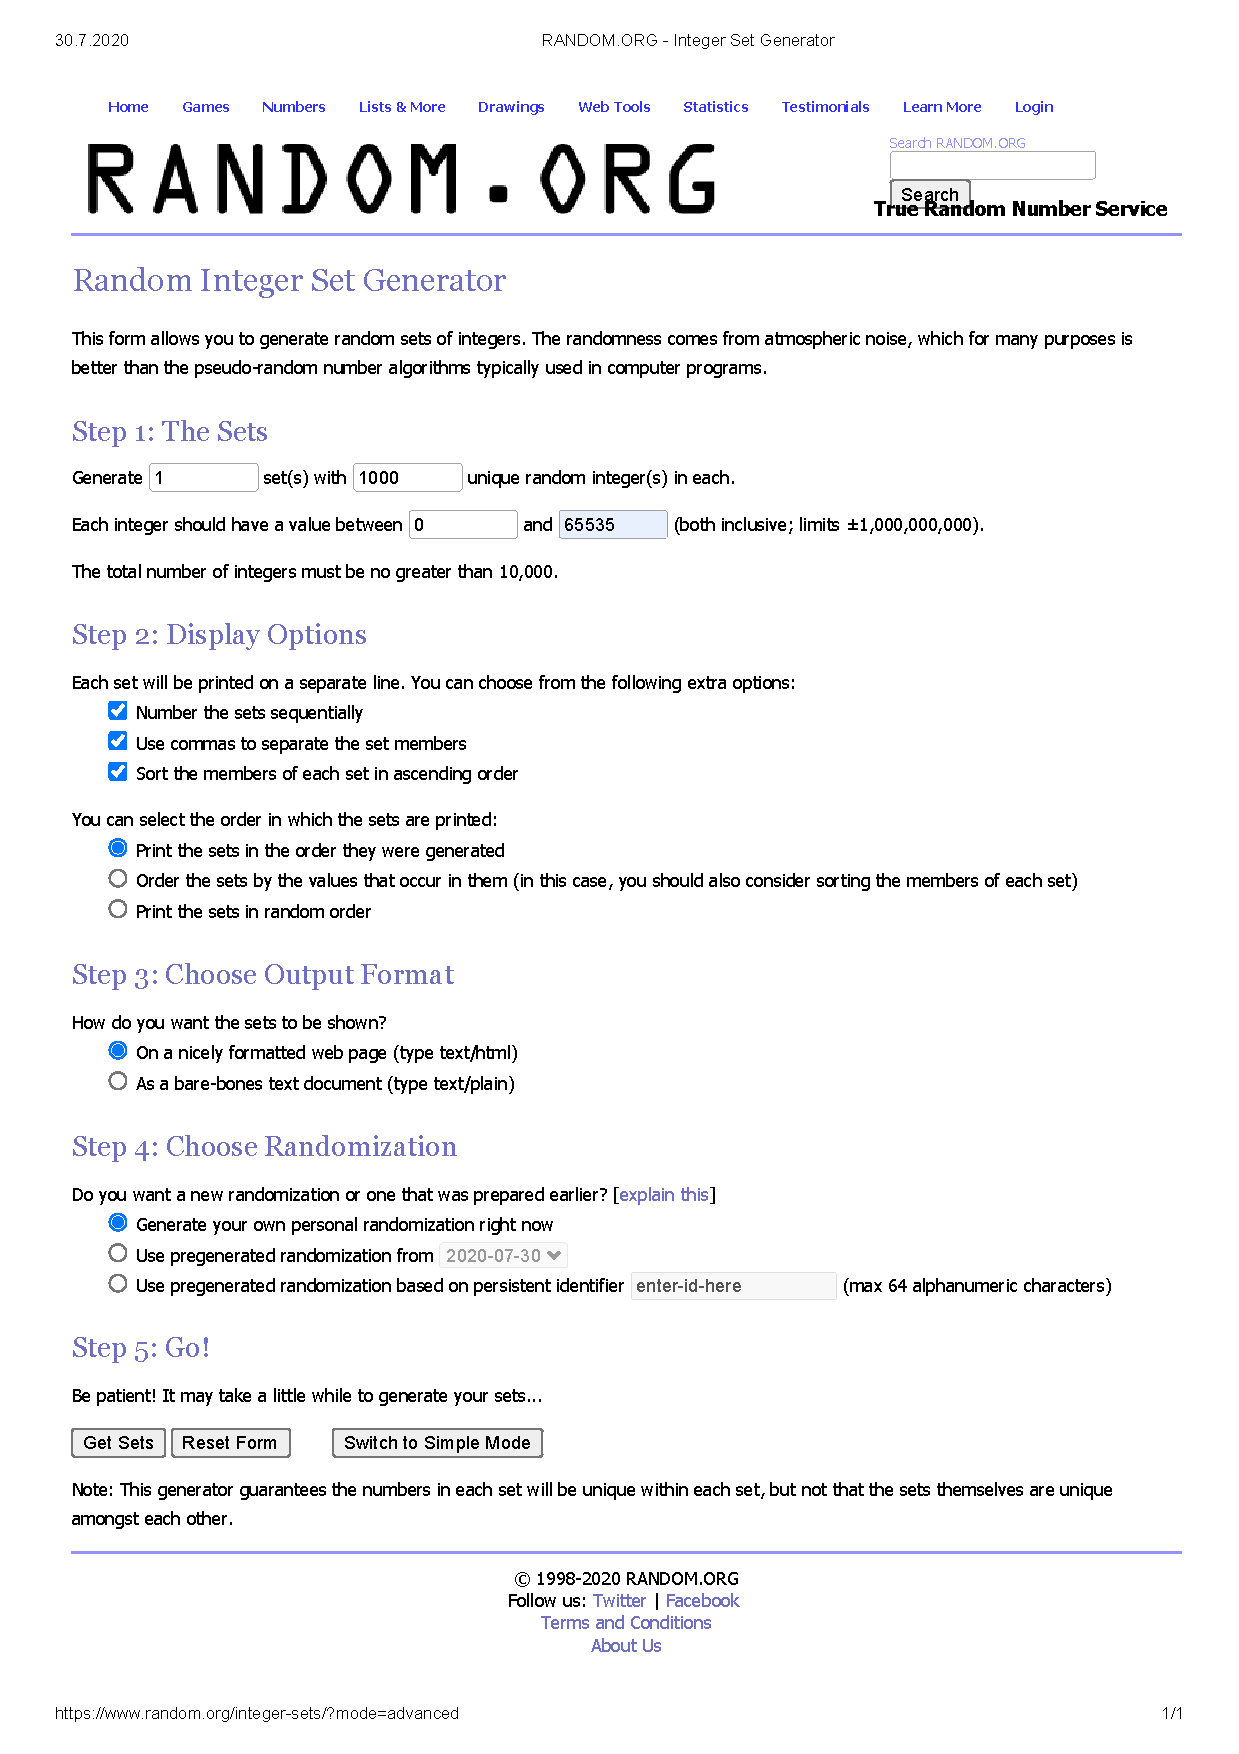
\includepdf[pages={1}, nup=1x1, landscape=false, scale=0.8 ,offset=0 -20, pagecommand={\section{Random Traffic Generation}\label{app:RandomTrafficGeneration}\thispagestyle{myheadings}}]{appendix/RANDOM.ORG_Integer_Set_Generator.pdf}


\end{appendix}



%%---NOTES for DEBUG---------------------------------------------------------------------
\ifdraft{%Do this only if mode=draft
%%requires \usepackage{todonotes})
\newpage
\listoftodos[\section{Todo-Notes}]
\clearpage
}
{%Do this only if mode=final
}

\end{document}
